% Do not forget to include Introduction
%---------------------------------------------------------------
%\chapter{Úvod}
% uncomment the following line to create an unnumbered chapter
\chapter*{Úvod}\addcontentsline{toc}{chapter}{Úvod}\markboth{Úvod}{Úvod}
%---------------------------------------------------------------
\setcounter{page}{1}

% The following environment can be used as a mini-introduction for a chapter. Use that any way it pleases you (or comment it out). It can contain, for instance, a summary of the chapter. Or, there can be a quotation.
Dotazníkové průzkumy patří dlouhodobě k nejjednodušším a nejužitečnějším nástrojům sloužících sběru dat. Kromě anket spokojenosti klientů s komerčními produkty, 
analýz volebních preferencí a jiných uplatnění nám tento zdánlivě přímočarý přístup umožňuje pochopit i celou řadu komplexních vlastností, které nás dělají lidmi. 
O slovo se potažmo hlásí psychologické a sociologické průzkumy, jež lze realizovat pomocí tzv. kompasových průzkumů.

Kompasovým průzkumem rozumíme dotazníkové šetření, jehož výstupem je graf rozdělený do čtyř kvadrantů. Tečky v takovém diagramu pak znázorňují jednotlivé účastníky 
daného průzkumu, jejichž odpovědi v dotazníku určují pozici příslušných teček. Tímto způsobem lze sledovat spoustu psychologicky a sociologicky 
zajímavých trendů – politické smýšlení ve středoškolských kolektivech, aktivitu/pasivitu studentů v různých oblastech jejich života, 
přístup k aktuálním světovým tématům atp.

Právě takové průzkumy bývají součástí rozsáhlejších projektů Somatopedické společnosti~\cite{Somspol2017}. Tato šetření umožňují zachytit stav vybraného 
sociologického nebo psychologického trendu před realizací intervenčních postupů, potažmo jeho stav po jejich ukončení. Na konci projektu může psycholog pomocí výstupů 
získaných z kompasového průzkumu porovnávat a tvořit z nich libovolné závěry.

Ovšem realizace kompasového průzkumu není efektivní – pro tvorbu dotazníku, jeho správu a následné vyhodnocení je nutné pracovat hned s několika softwarovými 
nástroji, které nejsou často pro osobu vedoucí průzkum dostatečně intuitivní, průzkumy jsou náchylné k chybám plynoucích z manuálního přístupu, a vzhledem ke 
komplexnosti přípravy dotazníku je třeba další osoby – analytika – který s danými nástroji umí pracovat a všechny podklady pro psychologa/sociologa připraví.

Zmíněným analytikem jsem já, proto jsem se rozhodl vytvořit nové softwarové řešení, které by mně a ostatním členům budoucích projektů celý proces usnadnilo. 
Zaměřením této bakalářské práce je tedy vývoj webové aplikace, která dokáže uspokojivě naplnit všechny kroky kompasového dotazníkového šetření.

V následujících kapitolách se budu věnovat detailněji aktuálnímu neefektivnímu řešení realizace kompasových průzkumů, sběru požadavků a softwarově inženýrskému návrhu 
prototypu nové aplikace. Praktická část bude pojednávat o samotné implementaci a následném testování použitelnosti aplikace při tvorbě pilotního průzkumu, 
které realizuji ve spolupráci s psychologem a několika dobrovolníky, kteří zaujmou roli respondentů tohoto testovacího šetření.


%---------------------------------------------------------------
\chapter*{Cíle a metodika}\addcontentsline{toc}{chapter}{Cíle a metodika}\markboth{Cíle a metodika}{Cíle a metodika}
%---------------------------------------------------------------

\section*{Cíle práce}\addcontentsline{toc}{section}{Cíle práce}\markboth{Cíle práce}{Cíle práce}
Hlavním cílem této bakalářské práce je navrhnout a implementovat prototyp webové aplikace, jenž umožní celý 
proces realizace kompasového průzkumu a to bez nutnosti intervence analytika nebo IT specialisty. 
Aplikace je tedy určena především pro psychology, sociology, pedagogy a jiné odborníky, kteří mají 
v úmyslu intuitivně sami realizovat kompasové dotazníkové šetření.

Pro dosažení hlavního cíle stanovujeme následující dílčí cíle:
\begin{enumerate}
    \item Analýza současného stavu – Zmapovat současné řešení problematiky kompasových průzkumů a určit jeho nedostatky.
    \item Analýza požadavků – Společně s psychologem a na základě zkušeností autora definovat konkrétní funkční a nefunkční požadavky na systém.
    \item Návrh nové aplikace – Provést softwarově inženýrský návrh aplikace a návrh uživatelského rozhraní.
    \item Implementace prototypu – Vyvinout prototyp aplikace odpovídající návrhu a pojednat o vybraných částech implementace. 
    \item Testování použitelnosti – Ověřit funkčnost prototypu s reálným uživatelem – psychologem se 
    zkušenostmi v oblasti kompasových dotazníkových šetření, vyhodnotit získanou zpětnou vazbu a navrhnout případná zlepšení.
\end{enumerate}

\section*{Metodika práce}\addcontentsline{toc}{section}{Metodika práce}\markboth{Metodika práce}{Metodika práce}
Metodický postup práce odpovídá klasickému postupu vývoje nového softwarového nástroje od úvodní rešerše 
klíčových technologií a přístupů, přes analýzu aktuálně používaného řešení až po samotný softwarově 
inženýrský návrh, implementaci a testování. Práce není tedy striktně rozdělena na teoretickou a praktickou část, 
nýbrž na jednotlivé na sebe plynule navazující kapitoly popisující ucelený proces návrhu a vývoje nové aplikace. 

Postup práce tedy lze rozdělit do následujících etap:
\begin{enumerate}
    \item Rešerše – Úvodní fáze ve které jsou popsány všechny důležité termíny a technologie 
    potřebné k pochopení ostatních částí práce.
    \item Analýza –  V této fázi jsou definovány konkrétní požadavky na systém na základě konzultace s 
    odborníkem a zkušeností autora, jenž se sám na realizaci kompasových průzkumů v minulosti aktivně podílel. 
    Formálně jsou zde definovány funkční a nefunkční požadavky, aktéři systému a případy užití.
    \item Návrh – Fáze návrhu navazuje plynule na provedenou analýzu. Zaměřuje se na návrh fyzické architektury systému, uživatelského rozhraní pomocí wireframů, 
    domény systému a konečně databázového modelu výsledné aplikace.
    \item Implementace – V této fázi je vyvíjen prototyp nové aplikace. Frontendová prezentační vrstva je úplně novou aplikací, zatímco backendový server je rozšířením a přepracováním aplikace, 
    kterou autor vyvíjel pro účely předmětu BI-TJV.
    \item Testování – Závěrečná fáze nutná k ověření funkčnosti nového softwarového řešení. Testování je provedeno s koncovými uživateli. Je sledováno zejména porozumění 
    testerů navrženému rozhraní a jejich zpětná vazba.
\end{enumerate}

%---------------------------------------------------------------

\chapter{Rešerše}
Cílem této kapitoly je pokrýt teoretický základ potřebný v dalších 
částech práce. To zahrnuje seznámení s problematikou komplexních 
dotazníkových šetření, s jejich terminologií a v neposlední řadě 
porovnání obdobných softwarových řešení. Zároveň jsou v této kapitole
představeny všechny klíčové technologie a přístupy potřebné k realizaci praktické
části práce.  

\section{Problematika dotazníkových šetření}
Dotazníkem rozumíme formulář určený nějakému respondentovi. Za jeho vynálezce
je běžně označován sir Francis Galton žijící v letech 1822–1911. První dotazníkový
průzkum, který byl výše zmíněným polyhistorem realizován, zkoumal dědičnost některých
lidských schopností. Galton dotazník sestavil a rozeslal ho 190 členům Královské společnosti.
Mezi otázkami, na které byli respondenti tázáni patřilo například jako kolikáté dítě se dotyční
narodili, jaké bylo povolání jejich rodičů a další.~\cite{jandourek2012slovnik}

Obecně je dotazník tvořen otázkami a několika uzavřenými možnostmi odpovědí, popřípadě
v některých případech ponechává místo pro zanechání odpovědi ve formě otevřeného textu.
V sociologickém výzkumu se jedná o velice populární způsob sběru dat, vzhledem k jednoduchosti
udržení kontroly reprezentativity a zpracování získaných dat.~\cite{jandourek2012slovnik}

Je nutné podotknout, že ačkoliv jsou pojmy \textit{„dotazník“} a \textit{„průzkum“}
často zaměňovány, existuje mezi nimi jistý rozdíl. Průzkumem rozumíme výzkumný přístup,
v rámci kterého jsou získávány subjektivní názory od vzorku subjektů, které jsou následně analyzovány.
Oproti tomu dotazník je metodou sběru dat využívaných v průběhu průzkumů, kde jsou respondenti
požádáni o odpovědi na předem definované sady otázek.~\cite{lau2017methods}

U dotazníků s uzavřenými možnostmi odpovědí může být respondent příliš omezen a je důležité,
aby byl takový průzkum proveden v prostředí, které daný výzkumník dobře zná.~\cite{jandourek2012slovnik}

Dobře sestavený dotazník je především jednoduchý na vyplnění. Dále by měl nejprve začínat
zajímavými otázkami na které respondent dokáže snadno odpovědět a až poté přejít k otázkám
méně zajímavým. Teprve ke konci dotazníku by měly být respondentovi představeny otázky citlivé
a osobní včetně identifikačních údajů. Nelze totiž opomenout skutečnost, že zodpovězení takových
otázek může ovlivnit odpovídání na další v pořadí.~\cite{jandourek2012slovnik}

\section{Kompasový diagram}
\label{subsection:compassdiagram}

\textit{Kompasovým diagramem} myslíme grafy, jejichž hodnoty nabývají formy teček umístěných v souřadnicovém systému. Ten je rozdělen na 4 kvadranty horizontální a vertikální linií, kde pozice teček vůči každé linii vyjadřuje naměřenou hodnotu jednoho respondenta dotazníkového šetření podle definovaného trendu. 

Co jednotlivé osy znamenají musí určit tvůrce průzkumu – pozice teček vůči osám může tedy například pro horizontální linii znamenat jak smýšlí jedinec ekonomicky, a pro vertikální linii zda se respondent kloní spíše k autoritářským nebo liberálním principům. Touto konkrétní implementací kompasového průzkumu se zabývá \textit{Politický kompas}~\cite{politicalcompass} zkoumající právě tyto sociologicé trendy. Politický kompas byl hlavní inspirací pro prvotní nápad uplatnění podobných diagramů i v jiných sociologických/psychologických problematikách. Na obrázku~\ref{fig:politicalcompass} lze vidět příklad kompasového diagramu v rámci Politického kompasu, jenž obsahuje odhady, jak by se v souřadnicovém systému mohli umístit někteří američtí politici, byli-li by respondenty takového dotazníkového šetření.

\begin{figure}[h!]
  \centering
  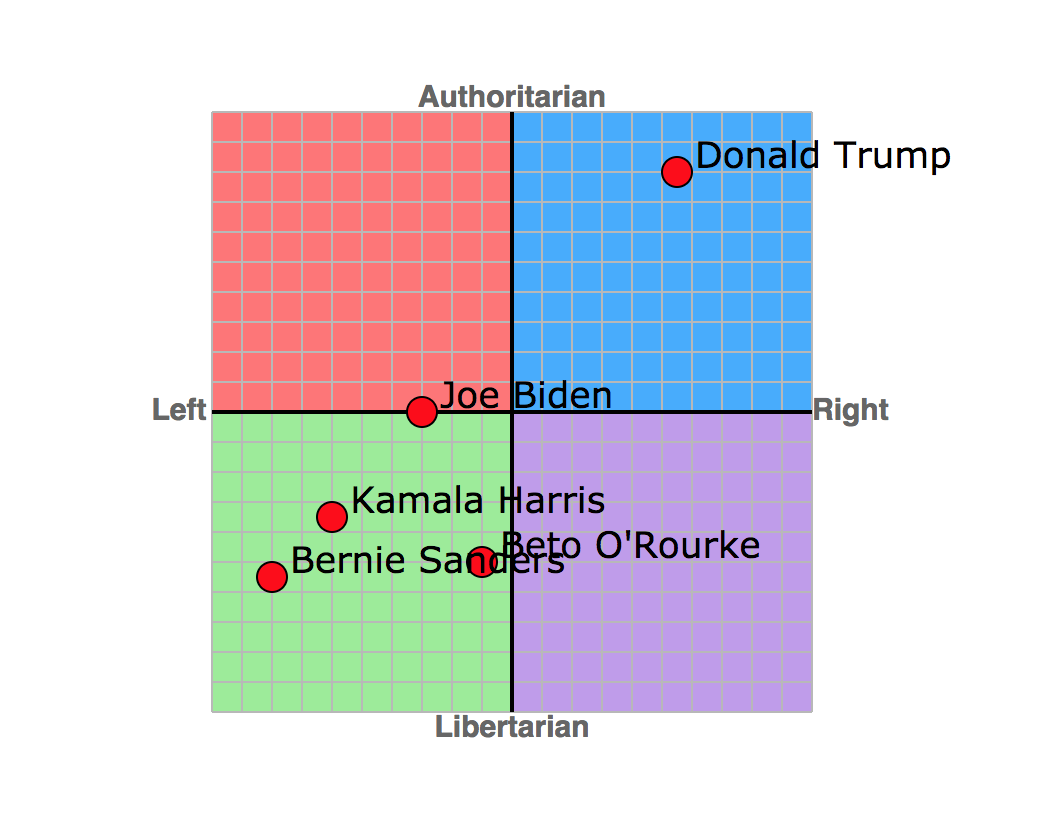
\includegraphics[width=\textwidth]{images/politicky_kompas.png}
  \caption{Politický kompas~\cite{politickykompaspng}}
  \label{fig:politicalcompass}
\end{figure}

Pro účely průzkumů uskutečněných pro Somatopedickou společnost byla metodika rozšířena o měření „průměrného respondenta.“ Do diagramu je tedy zahrnuta další od ostatních barevně odlišená tečka, jejíž pozice je definována jako průměr pozic všech ostatních teček v grafu.

Informace průměrném respondentovi nám mimo jiné poslouží i k výpočtu „soudržnosti“ zkoumaného kolektivu, tu chápeme jako průměr vzdáleností jednotlivých teček od pozice průměrného respondenta. Jednoduše řečeno to znamená, jak podobně daný kolektiv odpovídá v dotazníkovém šetření.

\subsection{Vyhodnocení kompasového průzkumu}
Samotné určení souřadnic teček reprezentujících respondenty v rámci kompasového diagramu
je založené na otázkách položených jako tvrzení. Účastník průzkumu u nich vyjádří
jak moc s danými tvrzeními souhlasí (vybere jednu z možností \textit{zcela souhlasí, spíše souhlasí, nevím, spíše nesouhlasí, zcela nesouhlasí}) – 
odpovědi jsou pak uloženy v číselných hodnotách: \textit{Zcela souhlasí = 1, spíše souhlasí = 0.5, nevím = 0, spíše nesouhlasí = -0.5, zcela nesouhlasí = -1.}
Každá hodnota je poté vynásobena \textit{váhou} příslušné otázky, tedy hodnotou určující jak moc
odpověď na danou otázku ovlivní výslednou pozici tečky v kompasovém grafu. Součet výsledných hodnot odpovědí na otázky příslušných
ke konkrétní ose je pak finální hodnota souřadnice ku této ose.

\section{Obdobná existující řešení}
Součástí vývoje nové aplikace je i pochopení kontextu dané problematiky, čemuž výrazně pomáhá i seznámení se s 
nástroji řešící stejnou či podobnou problematiku. Cílem následující rešerše je tedy poskytnout čtenáři přehled o 
podobných softwarových nástrojích pro tvorbu dotazníků, popsat jejich silné a slabé stránky a vhodnost jejich 
použití v kontextu realizace dotazníkových šetření.

Pro účely vývoje naší aplikace sledujeme u dotazníkových aplikací zejména jejich cenový model, přívětivost 
uživatelského rozhraní včetně dostupnosti v českém jazyce, možnost přizpůsobení otázek pro model kompasového 
průzkumu, schopnost aplikace validovat vstupy dle potřeb realizace kompasového dotazníkového šetření, možnosti
sdílení výsledného dotazníku s respondenty a schopnost správy odpovědí respondentů a jejich analýzy.

\subsection{Google Forms}
Google Forms je bezplatnou aplikací vyvinutou společností Google jako součást Google Workspace určenou pro 
snadnou a intuitivní tvorbu online formulářů. 

Rozhraní je čisté, intuitivní pro běžného uživatele, a plně přeložené do českého jazyka.

Během přidávání otázek do dotazníku aplikace umožňuje vybrat z několika typů otázek, včetně pro nás klíčového 
typu multiple choice. Otázky lze jednoduše uspořádat v přetahovacím rozhraní a výsledný dotazník pak sdílet s 
respondenty pomocí vygenerovaného odkazu, e-mailu, na sociálních médiích nebo vložením dotazníku na webu.

U otázek lze nastavit povinnost jejich vyplnění a kontrolu formátu (například zda je zadán platný e-mail). 
Také lze nastavit přesměrování respondenta na konkrétní otázky na základě jeho minulých odpovědí. 
Google Forms nabízí i efektivní správu a analýzu odpovědí – odpovědi lze v reálném čase pozorovat včetně 
jejich statistik, lze je následně exportovat do Google Sheets kde si uživatel může nastavit vlastní analýzu a 
její zobrazení.~\cite{googleforms}

Google Forms je součástí aktuálního řešení procesu realizace kompasových dotazníkových šetření, nicméně jeho 
nedostatky musí být kompenzovány začleněním dalších softwarových nástrojů do tvorby a správy dotazníků, 
což není vyhovující vzhledem k potřebě udržet práci dostatečně intuitivní, aby jí mohl obsloužit tvůrce průzkumu 
bez intervence IT specialisty nebo analytika. Těmito nedostatky jsou:

\begin{enumerate}
    \item Nedostatečná validace vstupů – Pro účely tvorby kompasových průzkumů je potřeba identifikovat 
    konkrétního respondenta dle jemu přiděleného identifikačního kódu. Také je třeba zabránit vícenásobnému 
    odeslání odpovědi, či odeslání odpovědi vydávající se za jiného respondenta. Ačkoliv Google Forms nabízí 
    některé základní způsoby validace vstupních hodnot, systém se nedaří přizpůsobit v takové míře, aby dostatečně 
    uspokojil tyto požadavky.
    \item Nemožnost tvorby kompasového diagramu – Vzhledem k tomu, že kompasový diagram je poměrně unikátním 
    způsobem zobrazení výsledku dotazníkového šetření, Google Forms jeho generování nativně neumožňuje. 
\end{enumerate}

\subsection{LimeSurvey}
LimeSurvey je open-source nástroj pro tvorbu dotazníkových průzkumů nabízející robustní systém známý 
svojí flexibilitou. Je dostupný ve dvou variantách – jako bezplatná Community Edition a jako bezplatná 
cloudová služba s několika úrovněmi předplatného. Oproti placené cloudové službě je u Community Edition 
nutné obstarat vlastní hostování aplikace.

LimeSurvey nabízí čisté moderní uživatelské rozhraní v českém jazyce umožňující poměrně intuitivní zacházení. 
Tvůrce průzkumu má na výběr z vícejak 28 různých typů otázek a více než 100 předpřipravených šablon pro snadné 
realizování různých typů dotazníkových šetření.

Typickou funkcí, která stojí za popularitou LimeSurvey, je flexibilita aplikace a možnosti nastavení pokročilé 
logiky a validace dotazníků pomocí funkce pro nastavení podmínek otázek. Tyto podmínky mohou upravovat logiku 
dotazníku na základě booleanovských operací, například porovnávání vstupního řetězce regulárními výrazy.

Správa účastníků průzkumu je oproti jiným podobným řešením velice flexibilní. Oproti základním funkcím správy 
respondentů a jejich sledování v reálném čase LimeSurvey umožňuje také generování unikátních přístupových kódů 
(tokenů) pro každého účastníka, automatické rozesílání připomínek respondentům, kteří ještě dotazník nevyplnili a 
nastavení tzv. kvót – omezení, kdo může odesílat odpovědi na dotazník například na základě pohlaví, věku či oblasti 
bydliště.

Vizualizace dat je v aplikaci možná prostřednictvím populárních grafů včetně sloupcových, koláčových,
prstencových a čárových diagramů. Nabízí i méně známé typy grafů, jako je radarový nebo polární graf.~\cite{LimeSurvey:online}

Pro účely kompasových dotazníkových šetření tedy LimeSurvey představuje velice robustního a vhodného 
kandidáta, avšak i toto softwarové řešení má několik nedostatků:

\begin{enumerate}
    \item Přilišná komplexnost aplikace – LimeSurvey je bezesporu velice flexibilním nástrojem, 
    ovšem vzhledem ke své robustnosti může uživatele spoustou možností zahltit. Přestože LimeSurvey dokáže 
    technicky obsloužit většinu požadavků na kompasové průzkumy, ztrácí tím uživatelskou přístupnost.
    \item Možná omezení ve verzi zdarma – Community Edition, bezplatná verze, může být místy omezená 
    oproti své placené variantě. Přestože LimeSurvey nabízí slevy pro studenty a neziskové organizace, 
    pro realizaci kompasových průzkumů dáváme přednost zcela bezplatným řešením.
    \item Nemožnost tvorby kompasového diagramu – Stejně jako Google Forms ani LimeSurvey nedokáže nativně 
    generovat kompasové diagramy přesně tak, jak bychom potřebovali.
\end{enumerate}

\subsection{Microsoft Forms}
Microsoft Forms je online nástroj pro tvorbu formulářů a dotazníků v rámci ekosystému Microsoft 365, 
z čehož plyne i jeho cena. Je navržený pro co nejrychlejší a nejjednodušší realizaci průzkumů s možností 
sběru a základní analýzy dat. 

Uživatelské rozhraní dostupné i v češtině je běžně uživateli označováno jako přehledné a jednoduché. 
Formulář je možné vytvořit do několika minut bez nutnosti hlubších znalostí.

Velkou výhodou oproti ostatním obdobným nástrojům je integrace s dalšími službami ekosystému Microsoft 365.

Uživatelé mají na výběr z několika základních typů otázek, mezi nimiž i typ multiple choice.

Správa odpovědí respondentů je velmi omezená, aplikace umožňuje zobrazit základní statistiky, ovšem už nenabízí 
tvorbu komplexnějších vizualizací dat.~\cite{Microsof74:online}~\cite{Jotformv14:online}

Klíčovými nedostatky Microsoft Forms jsou:

\begin{enumerate}
    \item Omezené možnosti validace vstupů – Podobně jako u Google Forms chybí možnost validovat 
    vstupy dle identifikačních kódů respondentů.
    \item Nemožnost tvorby kompasového diagramu – Nástroj umožňuje základní zobrazení, ovšem pro 
    komplexnější grafy, které jsou potřeba pro kompasová dotazníková šetření je nedostatečný.
    \item Aplikace není zdarma – Microsoft Forms je součástí Microsoft 365, je tedy nutné hradit placený plán, 
    aby bylo možné aplikaci vůbec využívat.
\end{enumerate}

\subsection{Shrnutí obdobných softwarových řešení}
Na tabulce~\ref{tab:similarsolutions} najdete přehled všech zkoumaných softwarových řešení pro tvorbu
dotazníkových šetření dle kritérií kompasových průzkumů.

\begin{table}[h!]
    \centering
    \renewcommand{\arraystretch}{1.2} % Zvýší výšku řádků pro čitelnost
    \begin{tabularx}{\textwidth}{|l|Y|Y|Y|}
        \hline
        \textbf{Kritérium} & \textbf{Google Forms} & \textbf{LimeSurvey} & \textbf{Microsoft Forms} \\ \hline
        Cena & Zdarma & Community Edition zdarma, placené plány & Součást Microsoft 365 (placené plány) \\ \hline
        Uživatelské rozhraní & Jednoduché, intuitivní & Komplexní & Jednoduché, intuitivní \\ \hline
        Dostupnost v českém jazyce & Ano & Ano & Ano \\ \hline
        Otázky & Základní & Více než 28 typů & Základní \\ \hline
        Validace & Základní & Pokročilá & Základní \\ \hline
        Sdílení & Odkaz, e-mail, sociální sítě, vložení na web & Odkaz, unikátní tokeny, kvóty & Odkaz \\ \hline
        Analýza & Základní statistiky & Široká škála grafů (sloupcové, radarové atd.) & Základní statistiky, integrace s Microsoft Excel \\ \hline
        Kompasový diagram & Ne & Ne & Ne \\ \hline
    \end{tabularx}
    \caption{Přehled obdobných dotazníkových nástrojů}
    \label{tab:similarsolutions}
\end{table}


\section{Technologie}
Cílem této sekce práce je seznámit čtenáře se všemi technologiemi a přístupy využitými k implementaci softwarového nástroje pro tvorbu kompasových průzkumů.

\subsection{REST}
REST je zkratkou pro \textit{„Representational State Transfer“} – styl softwarové architektury poprvé prezentované Royem Fieldingem v roce 2000. Od té doby se z něho stal jeden z nejrozšířeněji používaných přístupů vývoje webových API. 

Existuje mnoho cest, jak tuto architekturu implementovat, nicméně webové API nazveme REST API, nebo také RESTful API, pokud splňuje 5 základních principů:

\begin{enumerate}
\item REST API je uniformní a konzistentní rozhraní pro komunikaci mezi klientem a serverem – například REST API založené na HTTP/HTTPS komunikaci konzistentně využívá HTTP metod (GET, POST, PUT, DELETE, …) a URI (Uniform Resource Identifiers) pro identifikaci zdrojů,
\item Rozdělení na klienta a server – pro REST je důležitá filosofie rozdělení zodpovědností, což umožňuje aby obě části webové aplikace mohly být vyvíjeny odděleně,
\item bezstavovost – každý požadavek na server s REST API by měl obsahovat všechny informace potřebné k provedení žádané akce,
\item uložitelnost do mezipaměti (cacheble) – každá odpověď serveru by se měla sama označit za cacheble nebo non-cacheble. V prvním případě získává klientská aplikace právo data v odpovědi později znovu použít,
\item vrstvený systém – umožňuje architekturu aplikace členit hierarchicky. Stručněji řečeno, každá jednotka aplikace má přístup pouze do stejné a nižší vrstvy, než ve které se sama nachází. Příkladem takového vrstveného rozdělení povinností je návrhový vzor MVC.\cite{restfulapiWhatREST}
\end{enumerate}

\subsection{Specifikace OpenAPI}
\textit{Specifikace OpenAPI} je jazykově agnostickým dokumentačním rozhraním pro HTTP API systémy. Umožňuje snadné pochopení
služeb, aniž by bylo potřeba přistupovat ke kódu, webové dokumentaci, či jinému médiu a poskytuje tak snadnou, pro počítače i lidi srozumitelnou
cestu dokumentace vystavených koncových bodů aplikace.~\cite{OpenAPI}

\subsection{Spring Framework}
\label{subsection:spring}
\textit{Spring} je frameworkem založeným na programovacím jazyce Java. Nejdůležitějším prvkem tohoto rozhraní je pokrytí nízkoúrovňových požadavků výsledné aplikace tak, aby se vývojář mohl primárně soustředit na implementaci businessových operací. Spring tedy automaticky obstarává například správu závislostí (dependency injection,) autorizaci a autentizaci, zpracování požadavků a odpovědí prostřednictvím REST API, připojení k databázi a další.~\cite{spring}

Spring v této bakalářské práci zaujímá roli frameworku pro tvorbu backendové části aplikace. S jeho pomocí bude vystaveno REST API, se kterým bude prostřednictvím protokolu HTTP/HTTPS komunikovat frontendová část aplikace pro tvorbu kompasovách dotazníkových šetření.

\subsubsection{Spring Boot}
Pro urychlení vývoje a sestavení aplikace je v této práci využito nástroje \textit{Spring Boot}. Jde o jakousi nadstavbu nad samotným Spring frameworkem se zabudovaným serverem – Tomcat, Jetty, nebo Undertow – což umožňuje aplikaci jednoduše spustit jedním příkazem. Dále Spring Boot automatizuje konfiguraci aplikace, na rozdíl od samotného Springu tak není nutné upravovat žádné XML soubory za tímto účelem.~\cite{spring}


\subsection{Vue.js}
\label{subsection:vue}
\textit{Vue} je progresivní JavaScriptový framework užívaný zejména pro tvorbu uživatelského rozhraní. Je postaven na technologiích HTML, CSS a JavaScript. Vystavuje webovým vývojářům deklarativní programovací framework založený na tzv. \textit{„komponentách,“} které umožňují rozdělit uživatelské rozhraní do samostatných a znovupoužitelných kusů, přičemž jsou tyto komponenty běžně organizovány do stromové struktury, v níž jsou do sebe vzájemně dle potřeby zanořovány, jak ilustruje obrázek~\ref{fig:vuecomponent}.\cite{vue}

\begin{figure}[h!]
    \centering
    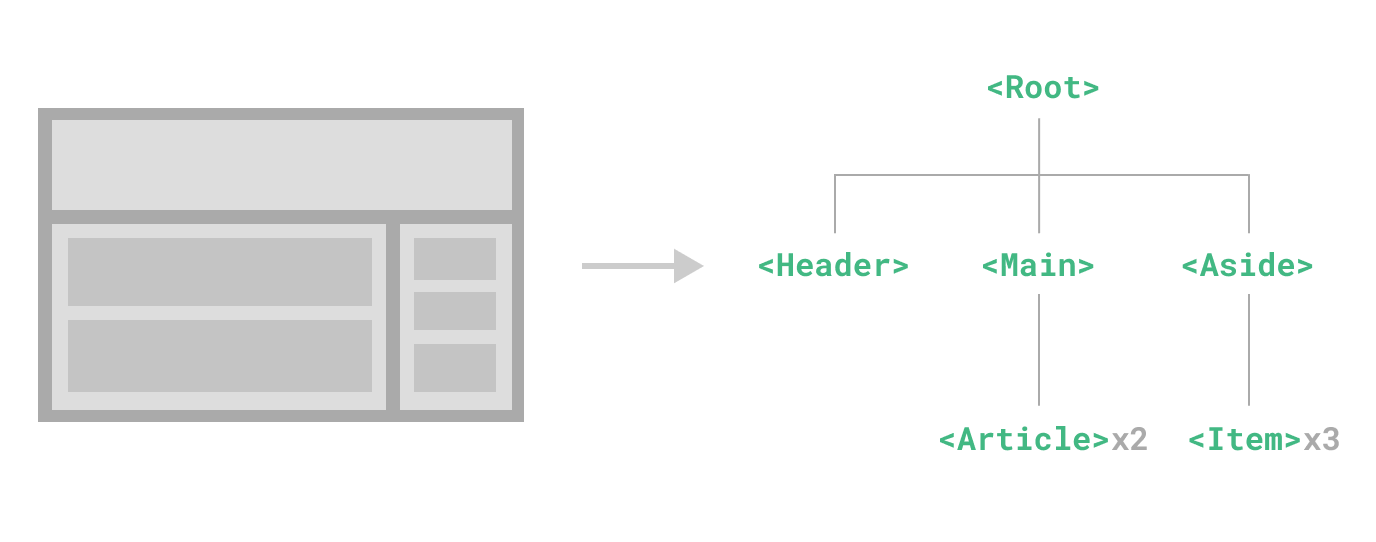
\includegraphics[width=\textwidth]{images/vuecomponents.png}
    \caption{Zanořování komponent ve Vue~\cite{vue}}
    \label{fig:vuecomponent}
\end{figure}

Klíčovými vlastnostmi technologie Vue jsou:
\begin{itemize}
    \item \textbf{deklarativní renderování} – Vue rozšiřuje standardní HTML šablonovým zápisem, čímž vývojářům umožňuje deklarativně popsat HTML výstup v závislosti na aplikačním JavaScriptovém stavu,
    \item \textbf{reaktivita} – Vue automaticky hlídá změny v JavaScriptovém stavu a aktualizuje jednotlivé prvky DOM hned, jakmile dojde ke změně.
\end{itemize}
V neposlední řadě je Vue velice flexibilním frameworkem umožňujícím širokou škálu přístupů k webovému frontendovému vývoji. Pro účely této práce je využit princip \textit{Single-Page Application} (SPA), tedy vývoj aplikace, kde si prezentační vrstva udržuje vnitřní logiku, díky níž frontendová aplikace dokáže dynamicky aktualizovat svůj stav bez nutnosti obnovovat stránku v prohlížeči při každé změně stavu aplikace. \cite{vue}

\subsection{Pinia}
\textit{Pinia} je oficiální Vue~(viz \ref{subsection:vue}) knihovnou pro správu stavu aplikace.
Umožňuje udržovat stav mezi více komponentami/stránkami. V kontextu aplikace pro tvorbu a správu dotazníkových šetření je 
Pinia využívána k udržení stavu předchozích požadavků na backendový server. Díky tomu je jednoduše možné, aby komponenta 
prezentující stav uživateli – například nějaký informační banner – měla přístup k výsledkům požadavků pramenících z komponent jiných.~\cite{pinia}

\subsection{Bootstrap}
\textit{Bootstrap} je široce používáným open-source frontendovým frameworkem určeným
k rychlému vývoji webových stránek a aplikací. Poskytuje spoustu předpřipravených komponent
implementovaných v HTML, CSS a JavaScriptu, což umožňuje vývoj výrazně urychlit. Velkou
výhodou používání Bootstrapu je zachování konzistence vzhledu vyvíjeného uživatelského
rozhraní.~\cite{bootstrap}

\subsection{Chart.js}
\label{subsection:chartjs}
\textit{Chart.js} je open-source JavaScriptovou knihovnou zaměřenou na tvorbu dynamických
a interaktivních grafů i dalších vizualizací. Nabízí celou řadu předpřipravených grafů od
těch nejzákladnějších jako jsou diagramy koláčové nebo sloupcové až po ty méně běžně používané.~\cite{chartjs}

Flexibilita tvorby grafů v Chart.js je klíčovou vlastností pro realizaci této bakalářské práce,
protože nabízí snadný způsob, jak programově tvořit kompasové diagramy.

\subsection{ORM}
\label{subsection:orm}
\textit{ORM (Object Relational Mapping)} je technikou používanou k vytvoření jakéhosi spojení
mezi objektově orientovanými programy a databázemi, především těmi relačními. Tento přístup
umožňuje vývojářům přistupovat k datům uložených v databázovém systému objektově místo nutnosti
ručního psaní SQL dotazů. To vývoj znatelně zjednodušuje a urychluje.~\cite{freecodecamp}

\subsubsection{Hibernate}
\label{subsection:hibernate}
\textit{Hibernate} je ORM nástroj umožňující vývojářům navrhovat třídy pro perzistenci dat
dle principů objektově orientovaného programování. To zahrnuje polymorfismus, dědičnost, kompozici a asociaci.
Hibernate je uznávaným nástrojem zejména díky své škálovatelnosti a výkonnosti.~\cite{freecodecamp}

Souběžně se svým nativním API Hibernate poskytuje konkrétní implementaci specifikace \textit{JPA (Jakarta Persistence API),}
která poskytuje množinu anotací a rozhraní pro práci s daty a jejich perzistencí.~\cite{hibernate}

\subsection{PostgreSQL}
\label{subsection:postgresql}
\textit{PostgreSQL} je relačně založeným databázovým systémem využívající rozšířeného dotazovacího jazyka SQL. Tento databázový systém je široce známý svojí spolehlivostí, jednoduchostí a vysokou škálovatelností. Systém je vlastněn a vyvíjen společností PostgreSQL Global Development Group, i přes to však zůstává kompletně open-source. Podporuje uživatelsky definované datové typy, což umožňuje efektivně využít databázi pro celou škálu obchodních modelů.\cite{postgresql} 

\subsection{OAuth 2.0}
Autorizační rozhraní \textit{OAuth 2.0} umožňuje autentizaci prostřednictvím třetí strany
v kontextu webových aplikací a nahrazuje dnes už zastaralý protokol OAuth 1.0.

V tradičním klient-server autentizačním modelu klient získá přístup k chráněným
zdrojům serveru prostřednictvím poskytnutím svých přihlašovacích údajů třetím stranám. Nicméně tento přístup je
z několika důvodů problematický:

\begin{itemize}
    \item Aplikace třetích stran musí ukládat údaje uživatele (vlastníka zdrojů) v čitelné podobě. Typicky se jedná o hesla.
    \item Servery musejí implementovat přihlašovací formuláře i přes bezpečnostní riziko plynoucí z vlastního ukládání hesel.
    \item Aplikace třetích stran získají zbytečně velký přístup ke zdrojům uživatele. A to bez možnosti vlastníka zdrojů 
    tento přístup časově či jinak omezit.
    \item Vlastníci zdrojů nemohou udělení přístupu ke svým údajům zrušit jedné třetí straně, aniž by tím zároveň nemuseli 
    přístup zrušit i všem ostatním třetím stranám.
    \item Pokud dojde k úniku hesel uložených třetí stranou, dojde ke komprimaci hesla konečného uživatele a všech dat chráněných tímto heslem.
\end{itemize}

OAuth všechny výše zmíněné problémy řeší separací role klienta a vlastníka zdrojů. Protokol představuje novou 
autentizační vrstvu – místo sdílení přihlašovacích údajů získá třetí strana \textit{přihlašovací token}, 
řetězec různý od přihlašovacích údajů uživatele umožňující serveru ověřit identitu přistupující strany.~\cite{oauth}

Diagram \ref{fig:oauth} znázorňuje typický postup dle protokolu OAuth 2.0.

\begin{figure}[h!]
    \centering
    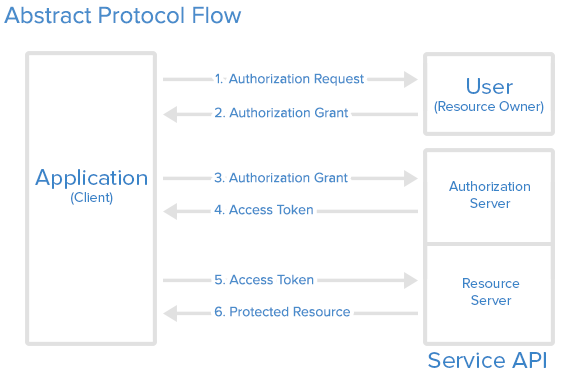
\includegraphics[width=\textwidth]{images/oauth.png}
    \caption{Proces autentizace dle OAuth 2.0~\cite{oauthimage}}
    \label{fig:oauth}
\end{figure}


\subsubsection{Keycloak}
\label{subsection:keycloak}
\textit{KeyCloak} je open-source řešení správy identit a přístupů v kontextu soudobých aplikací
umožňující jejich zabezpečení téměř bez nutnosti psaní vlastního kódu. KeyCloak poskytuje centralizované rozhraní 
pro správu uživatelů, autentizační služby, jednotné přihlášení (SSO), federaci identit a především
přihlášení dle protokolu OAuth 2.0.~\cite{keycloakreview}

V této bakalářské práci KeyCloak plní roli tzv. \textit{poskytovatele identit}, tedy 
autentizační vrstvy při protokolu OAuth 2.0.~\cite{keycloakdocs}
%---------------------------------------------------------------

\chapter{Analýza}
Analýza je kritickou součástí jakéhokoliv rozsáhlejšího softwarového vývoje. Jejím cílem je pochopení problému, pro který máme v úmyslu navrhnout řešení. To zahrnuje vymezení hranic navrhovaného systému, určení jaké požadavky jsou na něj kladeny, modelování domény a definování žádaného chování budoucí aplikace.

\section{Stávající řešení}
Cílem této části práce je vysvětlení současného přístupu správy a vyhodnocení dotazníků kompasových šetření a jejích klíčových nedostatků.

Tvorby kompasových průzkumů jsem se účastnil hned dvakrát. Poprvé v rámci projektu \textit{Na cestě k demokratické kultuře na střední škole} (2020) a podruhé při projektu \textit{Na cestě udržitelného rozvoje na střední škole} (2022). Obě iterace provázel téměř identický pracovní proces, který v následujících odstavcích popíši.

Nejprve je nutné stanovit, které trendy průzkum zkoumá – respektive co přesně znamená pozice teček (reprezentace odpovědí jednotlivých respondentů) vůči vertikální a horizontální ose kompasového diagramu. Například pro projekt \textit{Na cestě udržitelného rozvoje na střední škole} byla horizontální osa definovaná jako zájem/nezájem respondenta na základě jeho odpovědí, vertikální potažmo jeho pasivita/aktivita. (viz obrázek~\ref{fig:zajmovykompas})

\begin{figure}[h!]
    \centering
    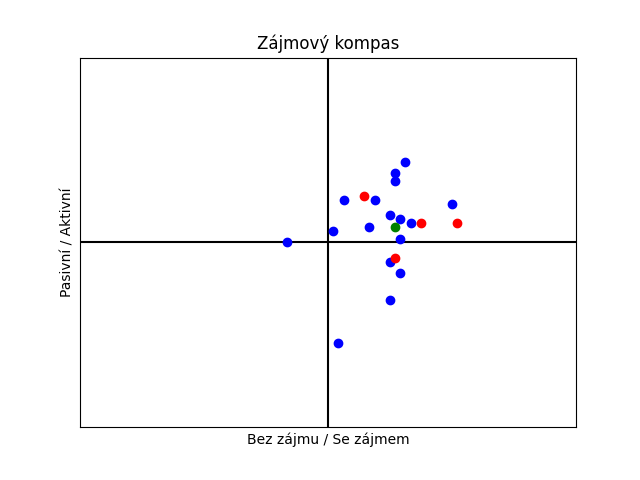
\includegraphics[width=\textwidth]{images/zajmovykompas.png}
    \caption{Příklad Zájmového kompasu, který umožnil měření respondentů v rámci zmíněného projektu}
    \label{fig:zajmovykompas}
\end{figure}

Dále musíme sestavit samotnou sérii otázek, které budou účástníkům průzkumu položeny. Tuto práci musí zastat člověk kvalifikovaný v daném oboru, jedná se tedy zejména o psychology a sociology. Dbát je nutné na způsob jakým jsou otázky položeny – například zda jsou dostatečně srozumitelné, či zda nejsou zavádějící. Zajímá nás také relevance otázek vůči zkoumané tématice. To vše musí tvůrce průzkumu vyhodnotit a otázky sepsat co nejvhodnějším způsobem.

Následně je seznam otázek předán analytikovi, tedy v případě minulých průzkumů přímo mně. Analytik otázky přepíše do nového dotazníku vytvořeného pomocí aplikace \textit{GoogleForms}~\cite{googleforms}. Každé otázce nastaví pět možných odpovědí – \textit{zcela souhlasím, spíše souhlasím, nevím, spíše nesouhlasím, zcela nesouhlasím}. Odkaz pro vyplnění dotazníku pak analytik zašle zpět tvůrci průzkumu. Celému dotazníku je pak nastaveno náhodné heslo, bez kterého ho není možné vyplnit. 

Mezitím tvůrce průzkumu poptá počet osob, které se budou dotazníkového šetření účastnit. Tato informace je dále předána analytikovi, jenž každému respondentovi přiřadí identifikační kód. Následně je sepsán dokument obsahující odkaz na průzkum, heslo k dotazníku a seznam všech identifikačních kódů. Celý tento dokument analytik předá psychologovi a ten jej odešle osobě dohlížející nad zkoumanou skupinou respondentů. Touto osobou byl v minulých průzkumech třídní učitel studentů, kteří byli účastníky dotazníkového šetření. Analytik dotazník otevře a v následujících dnech jsou respondenti požádáni o jeho vyplnění – pověřená osoba rozdá účastníkům průzkumu identifikační kódy, jimiž se do Google formuláře přihlásí.

V aktuálním přístupu neexistuje způsob, jakým bychom mohli zabránit odeslání chybně zadaného identifikačního kódu, případně jeho dvojímu odeslání. Analytik tedy musí průběžně odpovědi kontrolovat, nevalidní odpovědi promazávat a chybějící odpovědi vymáhat u učitelů, či jiných pověřených osob.

Jakmile jsou všechny odpovědi odeslány, analytik dotazníky uzavře a odpovědi si stáhne ve formě excelového souboru. Nyní je nutné ještě jednou manuálně zkontrolovat validitu všech odeslání. Analytik poté spustí python skript, který všechny tabulky analyzuje a vygeneruje příslušné grafy kompasů. Výsledný produkt skriptu společně s koláčovými grafy, které umožňuje vytvořit aplikace Google Forms, analytik zašle psychologovi, který hledá anomálie, zajímavé trendy a sepisuje závěrečný dokument.

\subsection{Nedostatky současného řešení}
V praxi se některé aspekty současného řešení ukázaly jako nevhodné. Zaprvé je nutné pracovat hned s několika softwarovými nástroji a organizace průzkumů se stává nepřehlednou a špatně udržitelnou – zejména provádíme-li více průzkumů najednou (například zkoumáme větší množství kolektivů v rámci jedné školy). Bylo by tedy vhodnější, kdybychom s průzkumy mohli pracovat v jediné centralizované aplikaci. Takový přístup je také řešením problému synchronizace dat mezi jednotlivými platformami.

Aktuální přístup vyplňování dotazníku skrze aplikaci Google Forms rovněž umožňuje jen velmi omezenou validaci vstupů zadaných účastníky průzkumu. Heslo pro přístup k dotazníku může být jen jedno pro celý zkoumaný kolektiv, což umožňuje účastníkům průzkumu, ať už záměrně nebo nezáměrně, odeslat odpověď dotazníku i za jiné osoby, jenž jsou součástí dotazníkového šetření. Částečně se tomu snažíme předejít identifikací účastníků pomocí přihlašovacích kódů. Ty jsou účastníkům rozdány společně s heslem k celému dotazníku. Ovšem identifikační / přihlaščovací kód je v průzkumu vyplňován jako odpověď na otevřenou textovou otázku, která už dále není nijak validována. Může se tedy stát, a na základě předchozích zkušeností k tomu dochází velice často, že účastník vyplňí identifikační kód špatně a je nutné, aby jej analytik manuálně zkontroloval a opravil, je-li vůbec poznatelné, který kód se respondent snažil vyplnit. Také nic nedokáže zabránit tomu, aby jeden respondent odeslal více odpovědí na jeden dotazník. Vývojem vlastní aplikace získáme naprostou kontrolou nad validací vstupů, kterou můžeme pro naše potřeby vhodně upravit. Přiřazením hesel každému účastníkovi zvlášť efektivně znemožníme neautorizovanému odeslání odpovědi.

Dalším problémem je nutnost intervence třetí osoby – analytika – pro úspěšnou realizaci dotazníkového průzkumu. Psycholog/sociolog totiž běžně není obeznámen se všemi potřebnými softwarovými nástroji. Analytik musí dotazník vytvořit v aplikaci Google Forms, odpovědi z dotazníku stáhnout ve formátu XLS/XLSX, odpovědi zkontrolovat, opravit a následně vyhodnotit prostřednictvím na míru napsaného skriptu v jazyce Python. Výsledkem vyhodnocení jsou kompasové diagramy a koláčové grafy, jež analytik musí předat tvůrci průzkumu. Centralizovaná a dostatečně intuitivní aplikace pokrývající všechny potřebné kroky dotazníkového šetření by však umožnila odstranění nutnosti intervence této třetí osoby – psycholog/sociolog by si vystačil se znalostí jediného softwarového nástroje.


\section{Analýza požadavků}
Na základě předchozích zkušeností a konzultací s psychologem, jenž se v minulosti na tvorbě kompasových průzkumů aktivně podílel, docházíme k následujícím požadavkům, které by měla nová aplikace pokrýt.
\subsection{Funkční požadavky}
\label{subsection:functionalreq}

\paragraph{FP.1 – Tvorba a správa dotazníků}~\\
Uživatel systému může tvořit nové dotazníky, přidávat a odebírat otázky, může dotazník otevírat a zavírat. Když dotazník uživatel otevře, dostane také odkaz a QR kód, který poté předá učiteli k rozdání mezi studenty. Je také nutné vygenerovat přihlašovací kód a jemu příslušné heslo pro konkrétního účastníka průzkumu.

\paragraph{FP.2 – Vyplnění dotazníku}~\\
Účastník se do dotazníku přihlásí pomocí přiděleného přihlašovacího kódu a hesla. Následně vyplní všechny povinné otázky a dotazník odešle.

\paragraph{FP.3 – Prohlédnutí a stažení získaných dat}~\\
Během průzkumu i po něm může uživatel systému prohlížet detaily již odeslaných odpovědí. Může si zobrazit jejich grafické reprezentace (tj. koláčové grafy a kompasový graf) a stáhnout si je jako obrázek.

\paragraph{FP.4 – Smazání získaných odpovědí}~\\
Získané odpovědi může uživatel smazat. Tato akce by měla být uživatelsky chráněna, aby bylo zabráněno mylnému smazání dat.

\subsection{Nefunkční požadavky}

\paragraph{NP.1 – Implementací je webová klient-server aplikace}~\\
Řešení pomocí webové aplikace volíme zejména z nutnosti snadného přístupu k aplikaci účastníky průzkumu.

\paragraph{NP.2 – Aplikace je robustní vůči chybám vstupů}~\\
Chyby vstupů mohou být například:
\begin{itemize}
    \item neplatné přihlašovací údaje účastníka průzkumu,
    \item odeslání odpovědí, aniž by byly všechny povinné vyplněny,
    \item duplikované zodpovězení otázky respondenta, který už dříve na danou otázku odpověď odeslal.
\end{itemize}

\paragraph{NP.3 – Dotazníky lze bez problému vyplňovat na mobilních zařízeních (frontendová aplikace je responzivní)
}~\\
Uživatelské rozhraní umožní pohodlné užívání aplikace bez ohledu na rozměry klientského zařízení.

\section{Případy užití}
\label{subsection:usecases}
Z funkčních požadavků vyplývají již konkrétní případy užití. Předtím, než budou všechny detailně popsány, je nutné definovat aktéry – uživatelské role v rámci vyvíjené aplikace pro tvorbu a správu dotazníkových šetření.

\subsection{Aktéři}
Aktéra, jenž má na starosti tvorbu a správu dotazníkových průzkumů nazveme \textit{Administrátor}. V praxi se jedná zejména o psychologa nebo sociologa.

\textit{Účastníka průzkumu} pak chápeme jako kohokoliv, komu je průzkum zadán k vyplnění. V kontextu této práce roli občas nazýváme \textit{„respondent“}. V minulých, už realizovaných projektech těmito účastníky byli nejčastěji například studenti středních škol, jejichž kolektiv byl předmětem sociologického průzkumu.

\subsection{Seznam případů užití}
\paragraph{UC.1 – Tvorba dotazníku}~\\
Aktér: Administrátor~\\
Uživatel vytvoří nový průzkum. Zvolí jeho název a libovolně přidává a upravuje otázky, u nichž volí jejich znění, jakou osu na výsledném kompasovém diagramu otázka ovlivňuje a s jakou vahou, přičemž je možné, aby byla hodnota vůči ose ovlivněna i záporně. Dále administrátor zvolí pořadí otázek.

\paragraph{UC.2 – Správa respondentů}~\\
Aktér: Administrátor~\\
Administrátor otevře průzkum, u něhož má v úmyslu spravovat respondenty. U konkrétního dotazníkového šetření zvolí počet respondentů, jaký si přeje obsloužit. Uživatel obdrží seznam dvojic obsahujících identifikační kód a heslo k přihlášení do dotazníku určených konkrétním respondentům. Respondenty je možné dodatečně přidávat i odstraňovat. Položka každého respondenta obsahuje informaci o tom, zda tento respondent již odeslal odpověď na průzkum.

\paragraph{UC.3 – Otevření/uzavření dotazníku k vyplnění}~\\
Aktér: Administrátor~\\
Uživatel otevře přehled průzkumu, který se chystá otevřít/zavřít. Po zvolení možnosti otevřít/zavřít dotazník je administrátor dotázán, zda tuto operaci skutečně chce uskutečnit. Je-li výzva potvrzena, dotazník změní svůj stav.

\paragraph{UC.4 – Správa odpovědí respondentů}~\\
Aktér: Administrátor~\\
Uživatel si zvolí průzkum, u kterého se chystá spravovat odpovědi. Po zvolení položky \textit{„odeslané odpovědi“} je přesměrován na stránku obsahující seznam všech respondentů, kteří průzkum vyplnili, odpověděli na všechny otázky. Uživatel zvolí respondenta a aplikace mu zobrazí jak daný účastník průzkumu odpověděl na každou otázku v dotazníku. Odpověď je možné smazat.

\paragraph{UC.5 – Vygenerování kompasového diagramu}~\\
Aktér: Administrátor~\\
Je-li průzkum uzavřen, uživatel u něj zvolí možnost \textit{„vytvořit kompas.“} Administrátor je dále dotázán, jak mají být jednotlivé osy v diagramu nazvány. Aplikace na základě odpovědí respondentů dotazník vyhodnotí a zobrazí vygenerovaný diagram, který je dále možné stáhnout na disk ve formátu PNG.

\paragraph{UC.6 – Vygenerování koláčového diagramu otázky}~\\
Aktér: Administrátor~\\
Je-li průzkum uzavřen, uživatel vybere možnost \textit{„statistika otázek.“} Následně je přesměrován na stránku obsahující vygenerované koláčové grafy popisující každou otázku. Administrátor si vybere, které grafy ho zajímají a ty stáhne na disk ve formátu PNG. 

\paragraph{UC.7 – Vygenerování údajů pro respondenty k rozdání}~\\
Aktér: Administrátor~\\
Uživatel zvolí průzkum a možnost \textit{„správa respondentů.“} Zde administrátor vybere \textit{„stáhnout dokument s respondenty“} a aplikace stáhne na disk soubor ve formátu PDF obsahující URL odkaz k vyplnění dotazníku, QR kód s výše uvedeným odkazem a seznam dvojic identifikačních kódů a k nim příslušných hesel.  

\paragraph{UC.8 – Vyplnění dotazníku}~\\
Aktér: Účastník průzkumu~\\
Jakmile uživatel obdrží svůj identifikační kód a heslo, zadá do svého prohlížeče URL adresu průzkumu k vyplnění, případně svým zařízením načte příslušný QR kód. Aplikace se dotáže na oba identifikační údaje, které respondent vyplní. Následně aplikace zobrazí otázky k vyplnění. Účastník průzkumu postupně odpovídá na otázky výběrem z několika možností. Jakmile má hotovo, uživatel zvolí možnost \textit{„odeslat.“}

\subsection{Diagram případů užití}
\begin{figure}[h!]
    \centering
    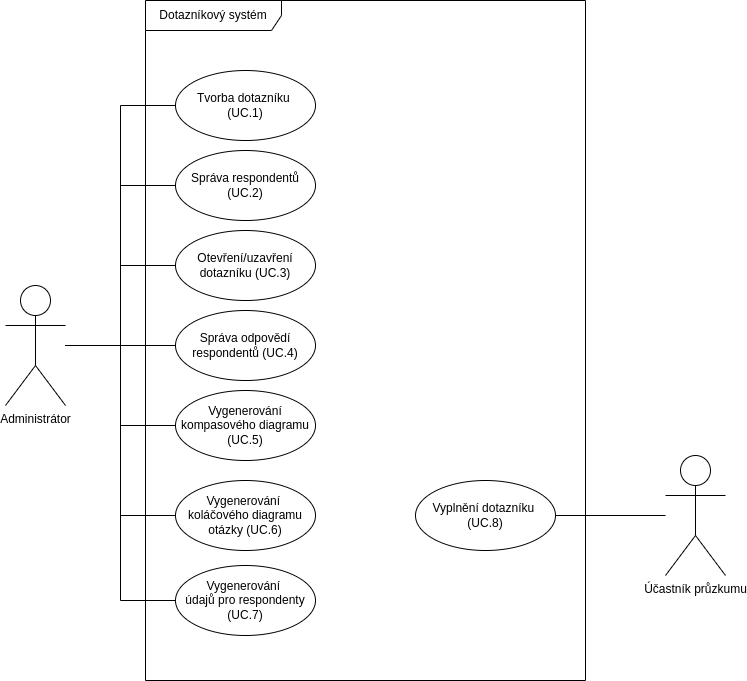
\includegraphics[width=\textwidth]{images/UCDiagram.png}
    \caption{UML diagram případu užití}
    \label{fig:umlusecase}
\end{figure}
%---------------------------------------------------------------

\chapter{Návrh}
Cílem této kapitoly je představit už konkrétní návrh nového softwarového řešení kompasových průzkumů.
Tato kapitola se zejména zabývá návrhem systémové domény, uživatelského rozhraní, databázového schématu a fyzického členění aplikace.

\section{Fyzická architektura}
Nové softwarové řešení je realizováno jako webová klient-server aplikace. 
Tento přístup byl zvolen, aby vyplnění dotazníku mohlo být jednoduše provedeno na 
jakémkoliv chytrém zařízení podporujícím některý z moderních internetových prohlížečů. 
Účastník průzkumu si zadá URL link do svého prohlížeče, případně načte QR kód obsahující
tentýž odkaz.

Aplikace je fyzicky dělena na čtyři části: frontendový server zajišťující interakci s 
uživateli a prezentaci dat, backendový server vystavující RESTful API pro komunikaci s 
prezentační částí aplikace, databázový server uchovávající stav všech průzkumů 
v systému a odpovědí respondentů, a konečně službu Keycloak (viz~\ref{subsection:keycloak}).

Do produkčního prostředí jsou pak všechny části aplikace kromě frontendu spuštěny pomocí Docker Compose.

\subsection{Frontend}
Prezentační server je implementován v technologii Vue (viz~\ref{subsection:vue}). Jedná se o moderní JavaScript framework umožňující snadný a intuitivní vývoj tzv. \textit{SPA (Single Page Application)} –  aplikací podporující \textit{„Fat Client“} princip, pro který je typický robustní frontend umožňující tvorbu dynamičtější a responzivnější aplikace, než kdybychom statické zdroje (JavaScript, HTML, CSS) generovali v backendové části aplikace, což by vyžadovalo znovunačtení všech zdrojů při každé změně stavu aplikace. 

Frontend komunikuje s backendovou částí pomocí HTTP/HTTPS protokolu skrze serverem vystavené REST API.

\subsection{Backend}
Backendový server vystavující REST API je implementován v technologii Spring (viz~\ref{subsection:spring}). 
Úlohou této části aplikace je provedení hlavních obchodních operací, přičemž každá z nich
začíná HTTP požadavkem přicházejícím z frontendové aplikace.

Pro práci s databází server využívá ORM nástroj Hibernate (viz~\ref{subsection:hibernate}) pomocí kterého
mapuje Java entity do tabulek relační databáze.

\subsection{Keycloak}
Keycloak služba je zprovozněna v samotném Docker kontejneru. Jejím smyslem je spravovat
uživatele systému a jejich zdroje a zároveň zaujímat roli identity providera v kontextu
protokolu Oauth 2.0.

Autentizace administrátora průzkumu tedy probíhá následovně:

\begin{enumerate}
    \item Frontendová aplikace prostřednictvím HTTPS požadavku předá přihlašovací údaje službě Keycloak.
    \item Keycloak údaje validuje a v případě úspěchu poskytne klientské aplikaci přístupový token.
    \item Frontend si token uloží a předává ho backendu v hlavičce každého požadavku.
    \item Backend token nejprve prostřednictvím HTTPS požadavku na Keycloak službu ověří legitimitu tokenu. Nenastane-li problém s validitou, backend provede očekávanou operaci.
\end{enumerate}

\subsection{Databáze}
Data aplikace jsou ukládána do PostgreSQL (viz~\ref{subsection:postgresql}) relační databáze, která je spuštěna ve svém Docker kontejneru.

Kromě dat samotné aplikace jsou zde uchována rovněž data služby Keycloak, jako jsou uživatelské účty administrátorů.

\section{Doménový model}
\label{subsection:domain}
Pro účely efektivního softwarového návrhu je vhodné nejprve modelovat \textit{doménu}.
Takový model slouží především k zachycení klíčových pojmů vznikající aplikace a vztahů
mezi nimi, což později usnadní návrh databázového schématu aplikace pro tvorbu dotazníků, i 
samotné navržení aplikačních objektů.

Doménový model na obrázku~\ref{fig:umldomain} přímo vychází z funkčních 
požadavků (\ref{subsection:functionalreq}) a případů užití (\ref{subsection:usecases}) a
odráží pochopení problematiky kompasových průzkumů v době návrhu aplikace.

Model na obrázku~\ref{fig:umldomain} je svým rozsahem abstraktní, nepopisuje technické detaily
budoucí implementace, jde pouze o prezentaci logických vztahů mezi entitami.

\begin{figure}[h!]
    \centering
    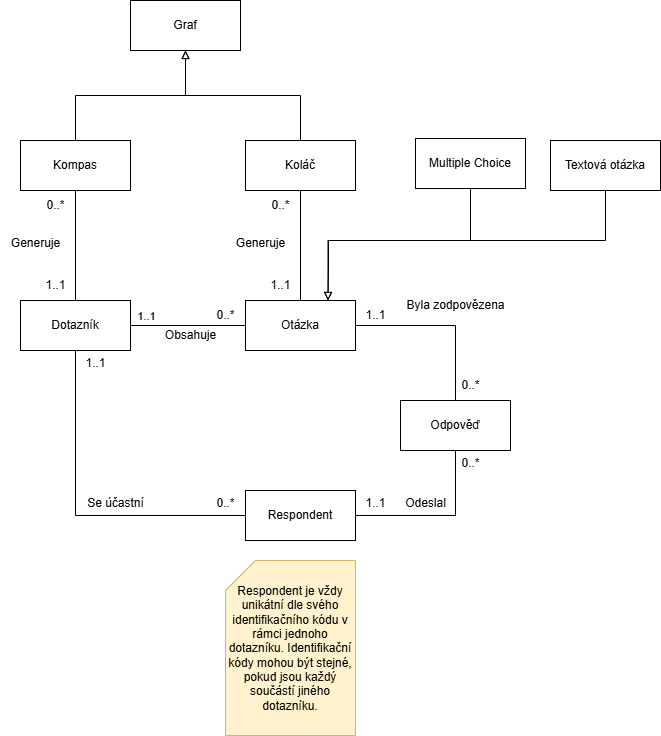
\includegraphics[width=\textwidth]{images/domain.drawio.png}
    \caption{UML diagram domény}
    \label{fig:umldomain}
\end{figure}

Pro jasné pochopení modelu následuje krátký popis všech entit uvedených v modelu:

\begin{itemize}
    \item \textbf{Dotazník} – Ústřední entita celé domény, abstrahuje jeden konkrétní průzkum vytvořený pro jeden kolektiv.
    Chceme-li například zadat stejný dotazník dvěma třídním kolektivům v rámci stejné školy,
    v doméně systému budou tyto dvě iterace vyjádřeny jako dva různé dotazníky.
    
    \item \textbf{Otázka} – Entita předávající respondentům informace, na základě 
    kterých odesílají odpovědi. V kontextu této domény může otázka být dvojího typu:
    \begin{enumerate}
        \item{Multiple Choice} – Jedná se o základní typ otázek kompasových průzkumů. Na otázku respondent odpovídá výběrem 
        jedné z několika možností: \textit{Zcela souhlasím, spíše souhlasím, nevím, spíše nesouhlasím
        zcela nesouhlasím.} V závislosti na odpovědích právě k tomuto typu otázek je později respondent 
        zobrazen na kompasovém diagramu.

        \item{Textová otázka} – Na tento typ otázek respondent odpovídá otevřeným textem. Není tak 
        důležitý jako otázky typu multiple choice, nicméně v rámci dotazníkových šetření může autorovi průzkumu
        poskytnout dodatečný vhled do dané problematiky.
    \end{enumerate}
    \item \textbf{Respondent} – Tato entita vyjadřuje jednoho účastníka průzkumu v rámci jednoho dotazníkového 
    šetření. V praxi se tak jedná například o studenty zkoumaného třídního kolektivu.
    \item \textbf{Odpověď} – Konkrétní vstup respondenta ve vztahu k jedné otázce průzkumu. Ukládá hodnotu zadanou respondentem.
    \item \textbf{Graf} – Entita graf je grafickým výstupem kompasového dotazníkového šetření 
    vznikající na základě již odeslaných odpovědí. Tyto diagramy slouží autorovi dotazníku jako materiál k tvorbě odborných závěrů. V kontextu systému rozeznáváme dva typy:
    \begin{enumerate}
        \item Kompas – kompasový graf je grafické vyjádření vyhodnocení všech respondentů dle jejich odpovědí na otázku typu multiple choice. (viz~\ref{subsection:compassdiagram})
        \item Koláč - koláčový graf vyjadřuje jak která část všech respondentů odpovídala na konkrétní otázku typu multiple choice.
    \end{enumerate}
\end{itemize}

\section{Databázový model}
\label{subsection:datamodel}
Pro konkrétnější přehled entit v rámci následné implementace byl na základě obecné
domény (viz~\ref{subsection:domain}) vytvořen databázový model~\ref{fig:datamodelnew} zobrazující konkrétní
tabulky včetně názvů jejich sloupců a datových typů databázového systému PosgreSQL.

Je patrné, že nezachycuje všechny entity z doménového modelu~\ref{fig:umldomain} vzhledem
k tomu, že není nutné všechny ukládat do databáze. Dalším důvodem
absence některých entit v databázovém modelu je, že jejich perzistence není 
řešena přímo vyvíjenou backendovou aplikací, například v případě entity \textit{Admin}, která
je spravována službou Keycloak tvořící si vlastní tabulky.

Entity generovaných diagramů není třeba ukládat do databáze, protože mohou být 
dynamicky tvořeny na základě entity \textit{Answer}.

\begin{figure}[h!]
    \centering
    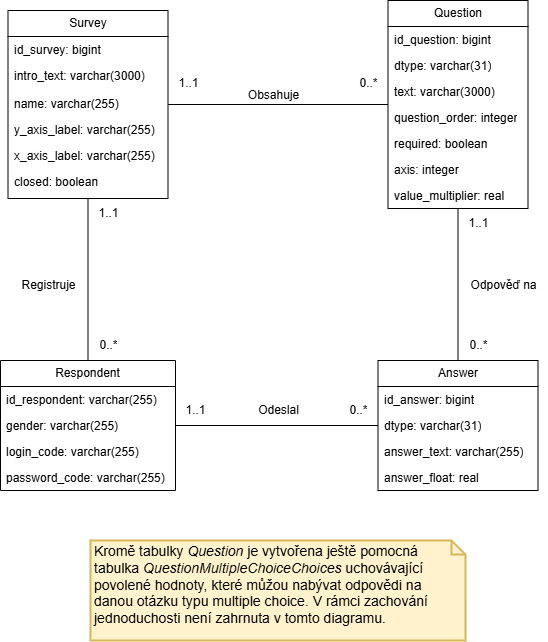
\includegraphics[width=\textwidth]{images/datamodel.drawio.png}
    \caption{Databázový model aplikace pro tvorbu kompasových průzkumů}
    \label{fig:datamodelnew}
\end{figure}

\section{Diagram aktivit}
Pro lepší pochopení procesů, které nastávají v průběhu realizace kompasových
dotazníkových šetření v kontextu nově vznikající aplikace
slouží UML diagram aktivit na obrázku~\ref{fig:activity}.

Diagram zachycuje činnosti od vytvoření nového dotazníku přes jeho distribuci, vyplnění
respondenty a konečně jeho analýzu. Tento pracovní postup je navržen z pohledu jednotlivých uživatelů.
Je nutné podotknout, že v rámci nového systému jsou uživateli aplikace pouze \textit{Administrátor} a \textit{Účastník průzkumu}.
\textit{Distributor} je pouze jakýmsi prostředníkem, který obdrží seznam přihlašovacích kódů a rozdělí je mezi účastníky průzkumu, nicméně
sám o sobě k aplikaci vůbec nepřistupuje.

\begin{figure}[h!]
    \centering
    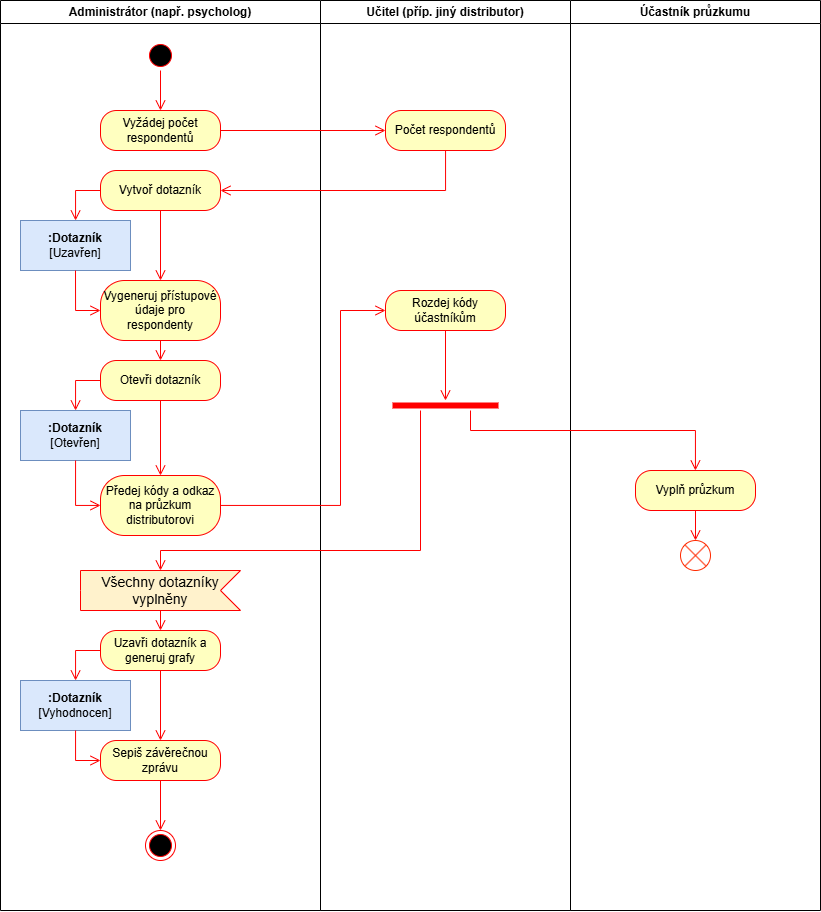
\includegraphics[width=\textwidth]{images/activity.png}
    \caption{Diagram aktivit provedení jednoho kompasového průzkumu}
    \label{fig:activity}
\end{figure}

\section{Stavový diagram entity dotazník}
Z diagramu aktivit~\ref{fig:activity} je zřetelné, že v průběhu dotazníkového šetření entita \textit{Dotazník}
nabývá 3 stavů. Tyto stavy a jejich změny znázorňuje detailněji stavový diagram~\ref{fig:state}.
\begin{figure}[h!]
    \centering
    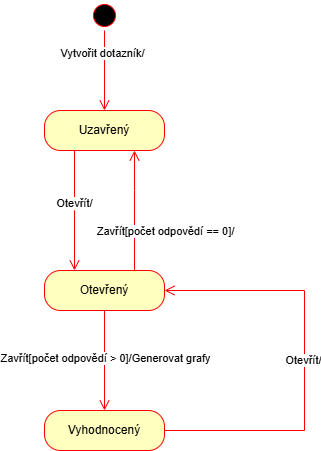
\includegraphics[height=\textwidth]{images/state.drawio.png}
    \caption{Stavový diagram entity Dotazník}
    \label{fig:state}
\end{figure}
Při svém vytvoření je dotazník uzavřen, tj. nepřijímá žádné odpovědi od respondentů. Jakmile
administrátor do dotazníku přidá otázky, nastaví úvodní text, pojmenuje osy X a Y a vygeneruje přístupové
kódy pro respondenty, je dotazník otevřen a přijímá odpovědi od účastníků průzkumu. Po obdržení všech odpovědí
administrátor dotazník opět uzavře a byla-li odeslána alespoň jedna odpověď na dotazník, automaticky proběhne
i jeho vyhodnocení prostřednictvím generováním popisných diagramů. Pak dotazník považujeme za vyhodnocený.
I vyhodnocený dotazník stále lze znovu otevřít, například potřebuje-li administrátor získat dodatečné odpovědi.

\section{Návrh uživatelského rozhraní}
Dobře navržené uživatelské rozhraní je klíčovým prvkem softwarového vývoje. Pro kompasová dotazníková
šetření jde o obzvlášť důležitou fázi vzhledem k tomu, že aplikace musí být dostatečně intuitivní
pro tvůrce dotazníkových šetření. 

Obecný postup návrhu tedy vypadal následovně:
\begin{enumerate}
    \item Nejprve byly pomocí online nástroje Mockflow vytvořeny prvotní \textit{wireframy} pro všechny
    logické stránky budoucího uživatelského rozhraní. Jedná se o zjednodušený návrh rozložení grafických
    prvků k zachycení základní struktury a funkčnosti jednotlivých obrazovek. Pomocí nich vznikla představa
    uživatelského rozhraní ještě před nutností vlastní implementace. Na obrázku~\ref{fig:wireframe1} najdete
    příklad jednoho z realizovaných wireframů. Zbytek návrhů je k dispozici v příloze~\ref{ap:wireframes}.
    Rozložení komponent ve wireframech vyplývá ze zkušeností autora při účasti na již realizovaných
    kompasových průzkumech.
    \item V návaznosti na výše uvedený hrubý návrh byl implementován prototyp pomocí CSS knihovny Bootstrap.
    Bootstrap byl použit především, aby bylo možné rychle vytvořit prezentovatelně vypadající prototyp.
    Během této implementace vyšly najevo některé nedostatky návrhu, například byly odstraněny některá grafická
    ohraničení, která nepřinášela funkční hodnotu, ale vizuálně znesnadňovala navigaci na obrazovce. Dále
    byla tlačítka s ikonami nahrazena textem, aby uživatelské rozhraní bylo jednoznačné i pro uživatele, kteří
    nejsou zvyklí na zaběhlé grafické normy. Na obrázku~\ref{fig:homescreenImplementation} lze vidět implementovaný prototyp 
    úvodní obrazovku aplikace zobrazující seznam všech průzkumů, které uživatel spravuje.
\end{enumerate}

\begin{figure}[h!]
    \centering
    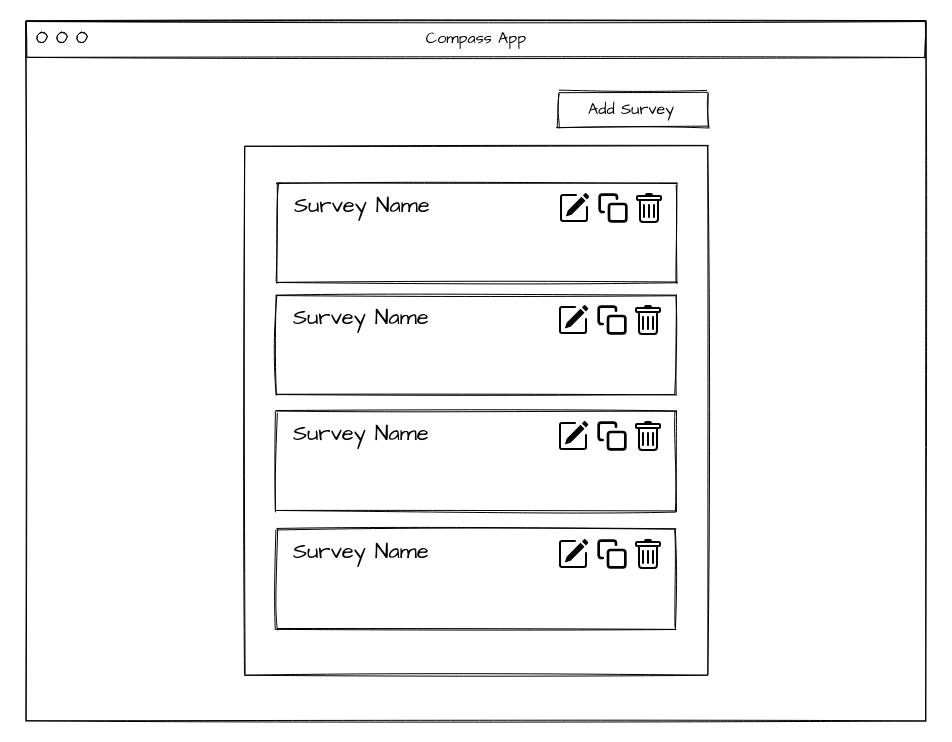
\includegraphics[width=\textwidth]{images/wireframes/Survey_List.png}
    \caption{Wireframe úvodní obrazovky}
    \label{fig:wireframe1}
\end{figure}

\begin{figure}[h!]
    \centering
    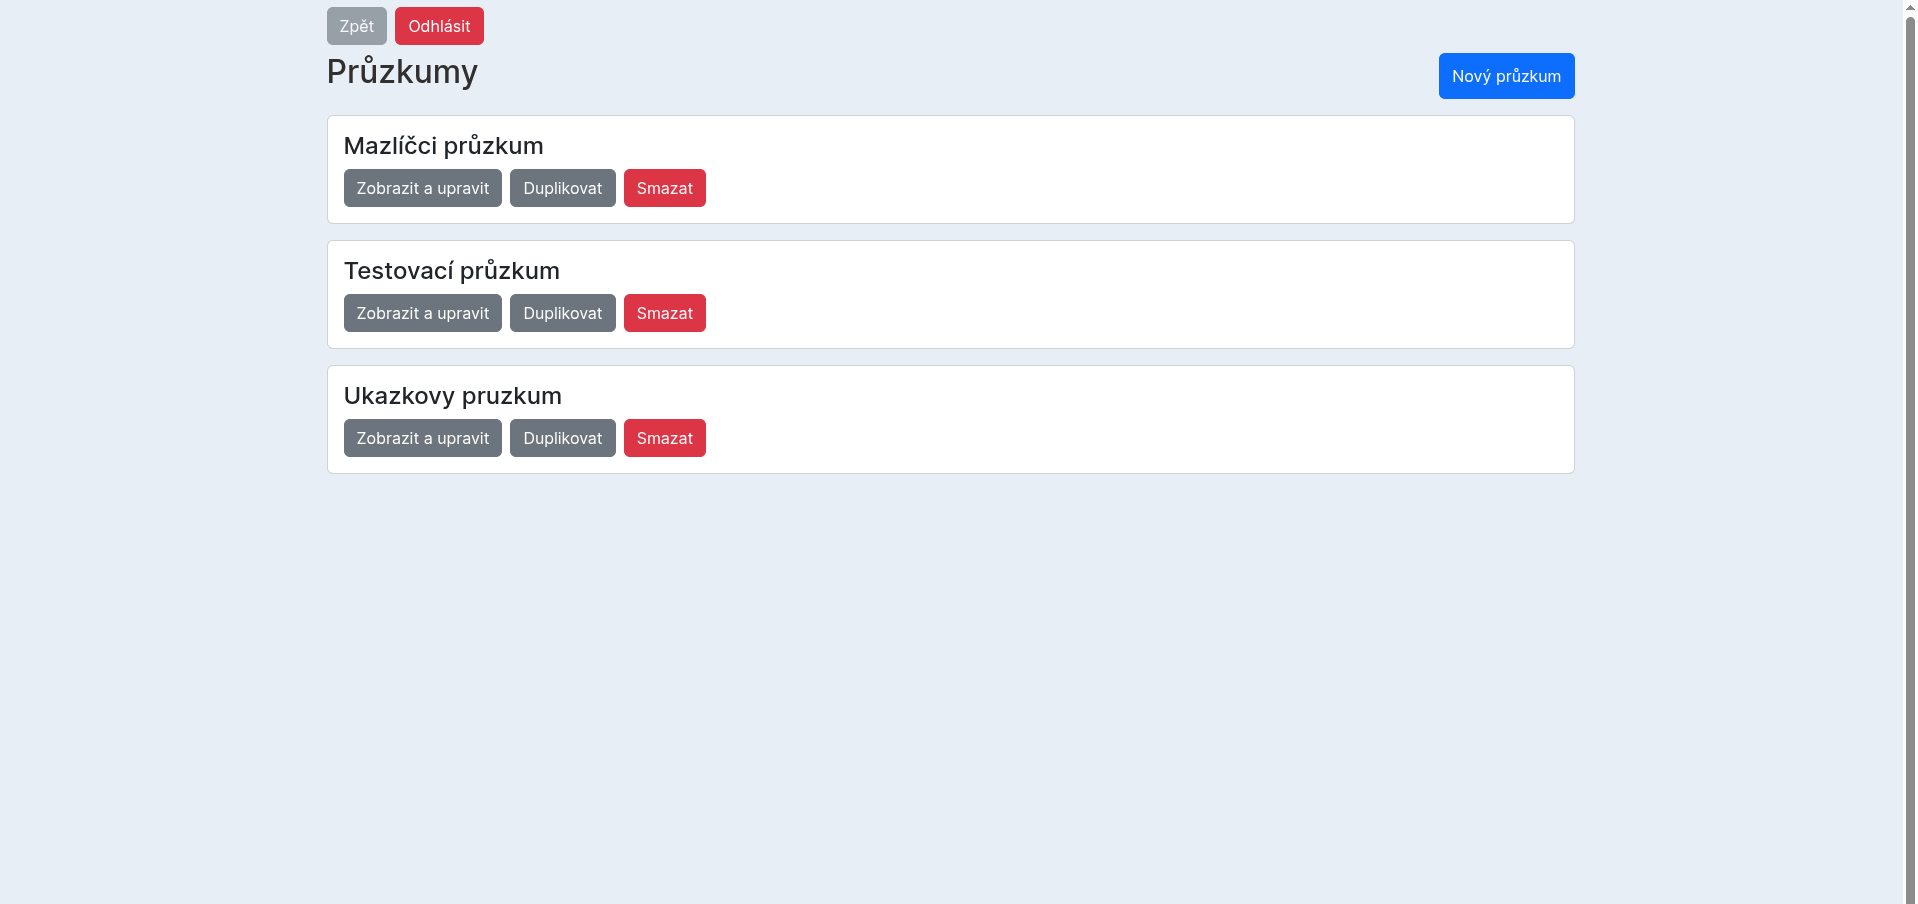
\includegraphics[width=\textwidth]{images/surveylistImpl.png}
    \caption{Implementace úvodní obrazovky}
    \label{fig:homescreenImplementation}
\end{figure}

Dalším krokem návrhu je jeho testování použitelnosti, na základě kterého jsou zjištěny nedostatky aktuálního
návrhu. Testování ovšem není předmětem této kapitoly a budeme se mu věnovat později v kapitole testování~\ref{subsection:testing}.
%---------------------------------------------------------------

\chapter{Implementace}
Implementace je kritickou fází vývoje jakéhokoliv softwaru. Jedná se o etapu,
během které abstraktní návrhy přecházejí v už konkrétní realizace. 
Tato kapitola se zaměřuje na vybrané části implementace aplikace pro tvorbu
kompasových dotazníkových šetření. Cílem je přiblížit čtenáři zajímavé body kódu jak
frontendové, tak backendové části. 

\section{Obecná struktura backendu}
Backendová část aplikace je vyvinuta v technologii Spring~(viz~\ref{subsection:spring}).
Její úlohou, jak bylo již zmíněno, je provést hlavní obchodní procesy definované funkčními
požadavky a případy užití.

Implementace byla navázána na semestrální práci pro předmět BI-TJV, jejímž
autorem je i autor této bakalářské práce. Doména původní práce byla velice jednoduchá a 
nepokrývala všechny požadavky, které jsou kladeny pro použitelnou aplikaci zaměřenou
na tvorbu kompasových průzkumů. Datový model popisující původní aplikaci je uveden na
obrázku~\ref{fig:originaldatamodel}.

\begin{figure}[h!]
    \centering
    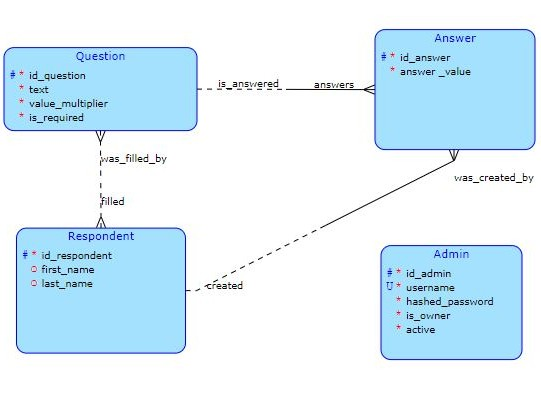
\includegraphics[width=\textwidth]{images/dataModel.JPG}
    \caption{Datový model původní práce}
    \label{fig:originaldatamodel}
\end{figure}

Doména pro účely nové aplikace byla tedy rozšířena, jak bylo popsáno v kapitolách Doménový model~\ref{subsection:domain}
a Databázový model~\ref{subsection:datamodel}.

Kód backendu je tedy členěn dle standardní třívrstvé architektury, kdy každá vrstva je závislá pouze na vrstvy stejné nebo nižší úrovně. 
Tato architektura členění kódu je klíčová pro přehledné rozdělení zodpovědností.

Nejvyšší vrstvou jsou třídy s anotací \textit{@Controller} jejíchž primárním účelem je distribuce práce mezi ostatní části aplikace.
Toto je místo, kde aplikace přijímá požadavky protokolu HTTP/HTTPS. Vzhledem k rozsahu aplikace a nedostatku času jsou některé třídy
s touto anotací nesprávně používány i k jiným účelům, to je do budoucna předmětem refaktoringu.

Další vrstvu tvoří třídy s anotací \textit{@Service}, představují služby, jejíž zodpovědností je provedení hlavní
obchodní logiky, tedy hlavních operací definovaných případy užití. Každá služba je
orientovaná na konkrétní část aplikace, zejména ve vztahu k jedné entitě domény.
Například zatímco třída \textit{RespondentService} se stará hlavně o tvorbu a správu
respondentů, zodpovědností třídy \textit{QuestionService} je obstarat otázky dotazníku a 
všechny operace s nimi související.

Nejnižší a poslední vrstvou je datová vrstva obsahující třídy s anotací \textit{@Repository}.
Tyto třídy jsou už přímo spjaty s perzistencí dat a prací s databází, ke které přistupují
prostřednictvím techniky ORM (viz~\ref{subsection:orm}). V implementaci této vrstvy
bylo využito rozhraní \textit{JpaRepository} z knihovny Spring Data JPA. To poskytuje
několik standardních metod obsluhujících tvorbu, úpravu a mazání dat 
bez nutnosti psaní vlastního kódu.

Pro všechny zmíněné vrstvy byla vytvořena abstraktní třída (\textit{AbstractCrudController, AbstractCrudService, CrudRepository}), ze které kontrolery, služby a 
repozitáře dědí a rozšiřují její funkcionalitu pouze o ty nutné pro práci
s danými entitami domény. Tento přístup zajišťuje přehlednost struktury kódu a rozšiřitelnost do budoucna.

\section{Obecná struktura frontendu}
Frontendová prezentační vrstva byla vyvinuta v rozhraní Vue (viz~\ref{subsection:vue}), ten umožňuje klientskou aplikaci
realizovat jako SPA (Single Page Application). Aplikace je rozdělena do komponent, tedy
samostatných celků zapsaných šablonovitým zápisem využívajících JavaScript/TypeScript, CSS a 
rozšířené HTML.

Základem architektury je komponenta \textit{App.vue} načtená do aplikace ve skriptu \textit{main.js}.
Tato kořenová komponenta obsahuje prvek \textit{<RouterView />} který dynamicky načítá ostatní komponenty
na základě aktuální URL adresy bez nutnosti statický obsah stahovat z backendového serveru. To vede k výrazně
plynulejšímu a rychlejšímu používání aplikace.

Každá Vue komponenta obsahuje 3 části:
\begin{itemize}
    \item <template> – vlastní šablonu v rozšířeném HTML zápisu,
    \item <script> – JavaScript/TypeScript kód obsluhující potřeby dané komponenty, 
    \item <style> – CSS styly.
\end{itemize}

Pro větší přehlednost a lepší organizaci kódu jsou komponenty ještě rozděleny na \textit{„views“} a \textit{„components“},
kdy první zmíněné zahrnuje komponenty představující jednotlivé stránky, každá odpovídající nějaké URL cestě.
Tyto komponenty jsou právě těmi, které jsou načítány ve Vue routeru definovaném v souboru \textit{src/router/index.ts}.
Komponenty v \textit{components} se pak skládají ze všech ostatních dílčích částí uživatelského rozhraní. 

\section{Autentizace službou Keycloak}
Aby byla aplikace zabezpečená a nebylo nutné implementovat vlastní systém autentizace a správy uživatelů,
je za tímto účelem využito open-source řešení Keycloak (viz~\ref{subsection:keycloak}). Služba je zprovozněna
jako server, na který frontendová i backendová část aplikace posílá HTTP/HTTPS požadavky za účelem ověření
identity uživatele. Jediný případ, kdy není nutná autentizace KeyCloakem je při vyplňování dotazníku,
vzhledem k tomu, že se jedná o část aplikace zpřístupněnou respondentům, kterým žádný administrátorský účet zřizován není.

Konfigurace komunikace mezi frontendovou aplikací a Keycloak serverem je realizována v souboru \textit{main.js} a je
zde představena v ukázce kódu~\ref{code:keycloak-init-fe}. Nejprve aplikace zjistí,
zda vyžádaná URL cesta odpovídá vyplnění dotazníku. Pokud ne, je uživatel přesměrován
na přihlašovací formulář Keycloak serveru. Po přihlášení je přesměrován zpět a proběhla-li
autentizace úspěšně, je celá Vue aplikace inicializována a získaný token uložen do lokálního uložiště.
Token je následně vkládán do hlavičky každého HTTP/HTTPS požadavku na backendový server.

\begin{listing}[h!]
    \begin{minted}[breaklines=true]{js}
const isSurveyFillRoute =
    window.location.pathname.startsWith("/survey/") &&
    window.location.pathname.includes("/fill");
keycloak
.init({ onLoad: isSurveyFillRoute ? "check-sso" : "login-required" })
.then((authenticated) => {
    if (authenticated || isSurveyFillRoute) {
    console.log("Authenticated");

    const app = createApp(App);
    const pinia = createPinia();

    app.use(router).use(pinia);
    const authStore = useAuthStore();

    authStore.setToken(keycloak.token);
    app.mount("#app");
    } else {
    console.warn("Not authenticated");
    window.location.login();
    }
})
.catch((error) => {
    console.error("Failed to initialize Keycloak", error);
});


    \end{minted}
\caption{Získání tokenu od Keycloak serveru}
\label{code:keycloak-init-fe}
\end{listing}

V backendové části aplikace je autentizace konfigurována ve třídě \textit{SecurityFilterChain} kde
je nastaven proces filtrace každého požadavku na server. V ukázce kódu~\ref{code:keycloak-init-be} lze nahlédnout
do tohoto nastavení. Jsou zde ručně specifikovány URL cesty, na které není potřeba autentizace. Zbytek cest pak
vyžaduje v hlavičce požadavku token, který je automaticky validován s Keycloak serverem. Ke Keycloak server je tedy v kontextu backendu
chápán jako identity provider protokolu OAuth 2.0.

\begin{listing}[h!]
    \begin{minted}[breaklines=true]{java}
   
@Bean
public SecurityFilterChain secConfig(HttpSecurity security) throws Exception {
    security
            .cors()
            .and()
            .csrf().disable() // Disable CSRF protection for simplicity
            .authorizeRequests()
            .antMatchers(HttpMethod.GET, "/swagger-ui/**").permitAll() // Allow documentation
            .antMatchers(HttpMethod.GET, "/v3/**").permitAll() // Allow documentation
            .antMatchers(HttpMethod.GET, "/respondent/survey/**").permitAll() // Allow GET requests to /survey/** without authentication
            .antMatchers(HttpMethod.POST, "/respondent/gender").permitAll()
            .antMatchers(HttpMethod.GET, "/respondent/*/finishedSurvey").permitAll()
            .antMatchers(HttpMethod.GET, "/question/**").permitAll()
            .antMatchers(HttpMethod.GET, "/survey/**").permitAll() // Allow GET requests to /survey/** without authentication
            .antMatchers(HttpMethod.POST, "/answer/**").permitAll() // Allow POST requests to /answer/** without authentication
            .antMatchers(HttpMethod.POST, "/survey/*/access/validate").permitAll() // Allow POST requests to /survey/*/access/validate without authentication
            .antMatchers(HttpMethod.OPTIONS, "/**").permitAll() // Allow CORS preflight requests
            .anyRequest().authenticated(); // All other requests require authentication

    security.oauth2ResourceServer(OAuth2ResourceServerConfigurer::jwt);
    return security.build();
}


    \end{minted}
\caption{Specifikace vyžádání ověření autentizace Spring aplikace}
\label{code:keycloak-init-be}
\end{listing}

\section{Komunikace s API}
Jak již bylo zmíněno v sekci pojednávající o obecné struktuře backendové aplikace, přístupové body aplikace jsou ve Spring aplikaci
definované v třídách s anotací \textit{@Controller}. V těch je definovaná cesta a HTTP metoda, která je obsloužena daným kontrolerem, když
backendový server obdrží příslušný požadavek.

Tyto požadavky pochází z klientské Vue aplikace a jsou na frontendu definovány v pro každou entitu příslušných souborech. Například pro entitu \textit{Question}
představující jednu otázku dotazníku jsou všechny potřebné požadavky definovány v souboru \textit{questionApi.ts}. Na ukázce kódu~\ref{code:readOneQuestionById} lze vidět příklad
požadavku na čtení jedné konkrétní otázky z backendového serveru dle jejího id.

\begin{listing}[h!]
    \begin{minted}[breaklines=true]{js}
async function fetchOneById(questionId: number) {
  try {
    const response = await apiClient.get(`/question/${questionId}`);
    return response.data;
  } catch (err) {
    console.error("Error fetching question:", err);
  }
}
    \end{minted}
\caption{Požadavek na získání jedné otázky dle jejího id}
\label{code:readOneQuestionById}
\end{listing}


\section{Pořadí otázek a jejich změna}
V rámci dotazníkových šetření může být pořadí otázek důležitým aspektem. Proto bylo třeba implementovat možnost
jejich pořadí ukládat a snadno měnit. V databázi tedy u každé otázky ukládáme i číselnou hodnotu \textit{questionOrder} vyjadřující jakousi
prioritu při řazení otázek – čím nižší číslo, tím je otázka výše. Když frontend otázky obdrží od backendového serveru,
na straně klienta je podle této hodnoty seřadí. Na ukázce kódu~\ref{code:moveQuestionDown} lze vidět implementaci funkce \textit{handleQuestionDown} která je volána
při stisknutí tlačítka pro posunutí otázky o 1 pozici níže. Seřazené pole otázek je postupně procházeno a když narazíme na otázku, kterou
chceme posunout v pořadí níže, index jí zvýšíme a případné sousední otázce ho naopak snížíme, tím otázky prohodíme. Obdobně jako tato funkce
funguje i funkce \textit{handleQuestionUp} pro posunutí otázky o jednu pozici výše.

\begin{listing}[h!]
    \begin{minted}[breaklines=true]{js}
const handleQuestionDown = async (question) => {
  let newArray = fetchedQuestions.value;

  newArray.forEach((q, index) => {
    if (q.id_question === question.id_question) {
      if (index + 1 < newArray.length) {
        // move down current question (raise index)
        let currentQuestion = newArray[index];
        currentQuestion.questionOrder = currentQuestion.questionOrder + 1;
        newArray[index] = currentQuestion;

        // move up next question (lower index)
        let nextQuestion = newArray[index + 1];
        nextQuestion.questionOrder = currentQuestion.questionOrder - 1;
        newArray[index + 1] = nextQuestion;

        // update question orders in API
        updateQuestionOrdersInApi(currentQuestion, nextQuestion);
      }
    }
  });

  fetchedQuestions.value = newArray;
  fetchedQuestions.value.sort((a, b) => a.questionOrder - b.questionOrder);
};

    \end{minted}
\caption{Funkce posunující otázku o jednu pozici níže}
\label{code:moveQuestionDown}
\end{listing}

\section{Dědičnost a databáze}
Během implementace ukládání otázek do databáze byl odhalen problém vztahující se k dědičnosti objektů. Databázový systém totiž 
nativně nepodporuje dědičnost entit, proto musí být třídy backendové aplikace nějakým způsobem namapovány do tabulek databáze.

Za účelem perzistence potomků třídy \textit{Question} (tedy konkrétně \textit{QuestionMultipleChoice} a \textit{QuestionOpenText}) byl zvolen přístup \textit{Single Table Inheritence}.
To znamená, že všechny entity se společným předkem jsou ukládány do jediné databázové tabulky obsahující všechny sloupce potřebné pro všechny potomky. 
Je-li pak některý sloupec pro uloženou entitu nerelevantní, je zde nastavena hodnota \textit{null}. Když později aplikace načítá objekty z databáze,
snadno pozná, o jakou konkrétní třídu se jedná na základě vyplněných sloupců.

Celou výše zmíněnou funkcionalitu Spring podporuje a je jí dosaženo jednoduše označením dotyčných entit anotací \textit{@Inheritence}, jak je
znázorněno v ukázce kódu~\ref{code:dedicnost}.

Tento přístup není ideální pro případy, kde existuje potenciál velkého množství derivovaných tříd společného předka, protože by pak
výsledná tabulka obsahovala příliš vysoký počet sloupců. Nicméně v našem případě se o velký problém nejedná, neboť pro účely kompasových
průzkumů jsou zcela nezbytné jen otázky typu multiple choice. Do budoucna by aplikace mohla ještě podporovat otevřené otázky, které jsou v backendové
části i implementované, nicméně vzhledem k rozsáhlosti vyvíjeného systému na tuto méně důležitou funkcionalitu nebyl čas a frontendová část pracuje
v době psaní této bakalářské práce pouze s otázkami typu multiple choice.


\begin{listing}[h!]
    \begin{minted}[breaklines=true]{java}
@Entity
@Inheritance(strategy = InheritanceType.SINGLE_TABLE)
public abstract class Question implements DomainEntity<Long>{ 
    (...)
}

    \end{minted}
\caption{Hlavička třídy entity Question}
\label{code:dedicnost}
\end{listing}

\section{Generování respondentů}
Než dotazník otevřeme respondentům k vyplnění, je nejprve třeba vytvořit pro dané respondenty jakési pseudoúčty obsahující identifikační
kód, podle něhož budeme moci sledovat, zda konkrétní účastník průzkum již dotazník vyplnil a náhodně vygenerované krátké heslo. Touto 
dvojicí údajů se pak subjekt průzkumu k dotazníku přihlásí, čímž zabráníme několikanásobnému odeslání odpovědi téhož respondenta, stejně jako
nežádoucímu odeslání odpovědi pod identitou někoho jiného.

Na ukázce kódu~\ref{code:respondents} jsou ukázány dvě klíčové metody generování přístupových dvojic (access pairs) tedy dvojic tvořených
z identifikačního kódu respondenta a desetimístného náhodného hesla. Metoda \textit{generateAccessPairs} nejprve spočítá už dříve vytvořené
respondenty k danému průzkumu. Dále každému respondentovi přiřadí identifikační kód sestávající z prvních tří písmen názvu průzkumu a pořadového čísla 
respondenta indexovaného od 0. Nakonec pomocí metody \textit{generatePasswordCode} vygeneruje náhodnou sekvenci 10 znaků, kterou uloží jako
heslo daného respondenta. Tyto přístupové dvojice jsou pak při odeslání odpovědi respondentem validovány.

\begin{listing}[h!]
    \begin{minted}[breaklines=true]{java}
private ArrayList<AccessPair> generateAccessPairs(int num, String survey_string, Long survey_id){
        ArrayList<AccessPair> pairs = new ArrayList<>();

        int respondent_count = ((RespondentRepository) repository).countAllBySurveyId(survey_id);

        for (int i = respondent_count; i < num + respondent_count; i++){
            String login_code = survey_string + i;
            String password_code = generatePasswordCode(10);
            pairs.add(new AccessPair(login_code, password_code));
        }
        return pairs;
    }

    private String generatePasswordCode(int len){
        SecureRandom random = new SecureRandom();
        StringBuilder password_code = new StringBuilder();
        for (int i = 0; i < len; i++){
            int index = random.nextInt(characters.length());
            password_code.append(characters.charAt(index));
        }

        return password_code.toString();
    }

    \end{minted}
\caption{Generování přístupových dvojic pro daný počet respondentů}
\label{code:respondents}
\end{listing}

\section{Odeslání odpovědí a rollback}
Když respondent vyplní všechny otázky a odešle dotazník, je volán koncový bod backendového serveru speciálně
určený pro vytvoření několik entit \textit{Answer} představující odpověď jednoho respondenta na jednu otázku.
Protože se však může stát, že nastane nějaká chyba během postupného zpracovávání jednotlivých odpovědí a není
žádoucí, aby v databázi byly v rámci jednoho dotazníku uchovávány pouze některé odpovědi a zbytek otázek zůstal
nezodpovězen, byla implementována funkce \textit{rollback}. Ta v případě chyby automaticky odstraní všechny již odeslané
odpovědi daným respondentem na otázky aktuálního dotazníku. Tato funkcionalita je znázorněna v ukázce kódu 
metody \textit{batchCreate}~\ref{code:batchcreate}.

\begin{listing}[h!]
    \begin{minted}[breaklines=true]{java}
@PostMapping("/batch")
    public Collection<AnswerDto> batchCreate(@RequestBody Collection<AnswerDto> dtos) {
    Collection<AnswerDto> answerDtos = new LinkedList<>();

    LinkedList<Long> submittedAnswerIds = new LinkedList<>();

    try{
        for (AnswerDto dto : dtos) {
            AnswerDto submitted = create(dto);
            answerDtos.add(submitted);

            submittedAnswerIds.add(submitted.getId_answer());
        }
    }
    catch (ResponseStatusException e){
        // If error, rollback answers
        for (Long id : submittedAnswerIds) {
            service.deleteById(id);
        }

        if (e.getStatus() == HttpStatus.BAD_REQUEST || e.getStatus() == HttpStatus.FORBIDDEN) {
            answerDtos.clear();
            throw new ResponseStatusException(HttpStatus.BAD_REQUEST, e.getReason());
        }
    }

    return answerDtos;
}

    \end{minted}
\caption{Metoda pro vytvoření odpovědí s funkcionalitou rollback}
\label{code:batchcreate}
\end{listing}

\section{Generování grafů}
Pro zobrazení konečných kompasových diagramů a koláčových grafů jednotlivých otázek 
bylo využito JavaScript knihovny Chart.js~(viz~\ref{subsection:chartjs}). Nicméně před samotným vykreslením diagramů
posílá klientská aplikace požadavek na Spring server, který údaje nutné k vykreslení
vhodně zpracuje. K tomu dochází v metodě \textit{readSurveyCompass}, která je v době psaní této práce dočasně
umístěná v třídě \textit{RespondentController} a její umístění je do budoucna předmětem refaktoringu. 

Získaná data pak frontendová aplikace dosadí do objektu \textit{chartOptions}, jenž předá
knihovně Chart.js dostatečné informace pro vykreslení kompasového diagramu.~\ref{code:chartoptions} Do objektu
\textit{chartData} jsou pak uložena konkrétní data respondentů, která jsou převedena na tečky v kompasovém grafu.

\begin{listing}[h!]
    \begin{minted}[breaklines=true]{js}
const chartOptions = ref({
  responsive: true,
  scales: {
    x: {
      title: {
        display: true,
        text: props.xAxisLabel,
      },
      type: "linear",
      position: "bottom",
      min: -10,
      max: 10,
      grid: {
        drawTicks: true,
        drawOnChartArea: true,
        drawBorder: true,
        color: (ctx) =>
          ctx.tick.value === 0 ? "rgb(179,179,179)" : "rgba(0,0,0,0.1)",
        lineWidth: (ctx) => (ctx.tick.value === 0 ? 2 : 1),
      },
    },

    ...}})
    \end{minted}
\caption{Příklad nastavení osy X objektu chartOptions}
\label{code:chartoptions}
\end{listing}

%---------------------------------------------------------------

\chapter{Testování}
\label{subsection:testing}
Testování je často podceňovanou fází softwarového vývoje. Slouží k ověření 
správnosti implementace a odhalení nedostatků které nebyly hned zřetelné během
samotného vývoje.

\section{Metodika testování použitelnosti}
V rámci vývoje aplikace pro tvorbu kompasových průzkumů bylo realizováno
především testování použitelnosti uživatelského rozhraní, jehož
cílem je ověřit pochopitelnost a snadnou použitelnost klientské části aplikace. 
Toto testování obsahovalo 3 fáze dle logického životního cyklu dotazníku:

\begin{enumerate}
    \item Tvorba dotazníku – Subjektem testu byl psycholog, jenž se v minulosti
    na realizaci kompasových průzkumů podílel.
    \item Vyplnění dotazníku – Test proběhl v několika iteracích s několika respondenty
    kteří plnili roli účastníka průzkumu.
    \item Analýza dotazníku – Subjektem byl opět psycholog, který se účastnil
    první fáze testu.
\end{enumerate}

Testerovi byly na začátku každé fáze nejprve zadány instrukce ke splnění konkrétního cíle
v závislosti na dané logické etapě. Dále byl tester srozuměn,
že předmětem testování nejsou jeho schopnosti, nýbrž aplikace samotná a případné
chyby či nesrovnalosti by neměly být zdrojem testerova znepokojení. Tester byl
také požádán, aby své myšlenkové vzorce ohledně práce s aplikací vokalizoval nahlas.

Následně byl test spuštěn a bylo na testerovi, zda dokáže splnit stanovené instrukce
bez intervence přihlížejícího autora této práce. Zatímco subjekt plnil úkoly,
autor pozoroval testerovo chování a dělal si poznámky ohledně jeho nejasností 
a nedostatcích, která vyšla najevo.

Po ukončení testu byly poznámky analyzovány, sepsány a bylo navrženo jejich možné řešení.

\section{Tvorba dotazníku}
Tato fáze testu použitelnosti pokrývá následující případy užití~(viz~\ref{subsection:usecases}):

\begin{itemize}
    \item UC.1 – Tvorba dotazníku
    \item UC.2 – Správa respondentů
    \item UC.3 – Otevření/uzavření dotazníku
    \item UC.7 – Vygenerování údajů pro respondenty
\end{itemize}

Psycholog, jenž byl v této fázi testerem, obdržel následující instrukce:

\begin{enumerate}
    \item Vytvořte nový průzkum.
    \item Nastavte název průzkumu.
    \item Vyplňte úvodní text průzkumu.
    \item Přejmenujte osy X a Y podle Vašich metrik.
    \item Přidejte do průzkumu Vaše připravené otázky a správně
    je nastavte dle jejich působení na osy X a Y.
    \item Vygenerujte kódy pro 10 respondentů.
    \item Stáhněte PDF dokument obsahující údaje pro respondenty.
    \item Zpřístupněte dotazník k vyplnění.
\end{enumerate}

\section{Vyplnění dotazníku}
Fáze vyplnění dotazníku pokrývá případ užití UC.8 – vyplnění dotazníku.

V rámci první fáze testu byly vygenerovány přístupové kódy pro
celkem 10 respondentů. Roli každého z nich plnil odpovídající počet dobrovolníků.

Každému testerovi byly zadány následující instrukce:

\begin{enumerate}
    \item Načtěte stránku s průzkumem přes odkaz nebo QR kód.
    \item Vyplňte vám přidělený identifikační kód a heslo.
    \item Vyplňte všechny otázky v dotazníku.
    \item Odešlete dotazník.
\end{enumerate}

\section{Analýza dotazníku}
Poslední fáze testu použitelnosti pokrývá tyto případy užití:

\begin{itemize}
    \item UC.2 – Správa respondentů
    \item UC.3 – Otevření/uzavření dotazníku
    \item UC.4 – Správa odpovědí respondentů
    \item UC.5 – Vygenerování kompasového diagramu
    \item UC.6 – Vygenerování koláčového diagramu otázky
\end{itemize}

Testerem v této fázi testu byl tentýž psycholog, který dotazník vytvořil
v rámci první fáze testu použitelnosti.

Psychologovi byly zadány následující instrukce:

\begin{enumerate}
    \item Zkontrolujte, zda všichni respondenti dotazník vyplnili.
    \item Uzavřete dotazník.
    \item Zkontrolujte, jakou možnost vybral první respondent s pořadovým číslem 1
    na druhou otázku dotazníku.
    \item Stáhněte koláčový graf této otázky.
    \item Stáhněte kompasový diagram průzkumu.
\end{enumerate}

\section{Klíčové nedostatky a návrh jejich řešení}
Následuje seznam klíčových nedostatků dle poznámek autora na základě testu
použitelnosti včetně návrhu na jejich zlepšení do budoucího vývoje
aplikace pro tvorbu kompasových dotazníkových šetření.

\paragraph{Priorita tlačítek}~\\
V některých částech aplikace testera dostatečně vizuálně neupoutalo
tlačítko pro logické pokračování v seznamu instrukcí. Tímto způsobem
problematické je například tlačítko \textit{„nový průzkum“}, které se poněkud
ztrácí mezi položkami již existujících dříve vytvořených průzkumů. Tester
pak měl tendenci spíše upravovat tyto průzkumy, než aby vytvořil nový.

Řešením je zvýšit vizuální atraktivitu tlačítka, mělo by být větší a čitelnější.
Také je vhodné tlačítko přesunout někam ke středu obrazovky, aby si jej uživatel
všiml dříve, než položek existujících průzkumů.


\paragraph{Logická návaznost kroků}~\\
Tester se často dostával do situací, kdy si nebyl jistý, na co by měl dále kliknout. 
Stránka nastavení průzkumu se ukázala jako špatně přehledná vzhledem k množství komponent
a neintuitivnímu rozložení tlačítek.

Řešením je vytvoření samostatné stránky pro každý krok tvorby dotazníku, čímž by
se proces proklikávání aplikace stal mnohem lineárnějším a jednoznačnějším. Vhodné by tedy
bylo nejprve uživateli nabídnout změnu jména a úvodního textu průzkumu, poté změnu názvu os diagramu,
dále by měla následovat stránka spravující otázky průzkumu a nakonec správa respondentů a uzavření
průzkumu.


\paragraph{Určení váhy otázky}~\\
Váha otázky v kontextu kompasových průzkumů vyjadřuje, jak moc a kterým směrem daná otázka
ovlivňuje pozici výsledné tečky na dané ose. Přístup otevřeného číselného pole, kam uživatel
zadává libovolnou hodnotu se ukázal být zbytečně liberálním a velice neintuitivním. Tester 
si s touto částí nastavení otázky vůbec nevěděl rady.

Řešením je počet možností, jak nastavit váhu otázky omezit a její jednotlivé hodnoty intuitivně pojmenovat.
Místo číselného pole by tedy uživatel měl na výběr z několika slovy pojmenovaných důležitostí otázky,
například \textit{nízká, střední, vysoká}. Dále je vhodné přidat zatrhávací možnost, jakým směrem otázka osu ovlivňuje.

\paragraph{Pojmenování os}~\\
Když měl tester určit pojmenování jednotlivých os kompasového diagramu,
byl zmatený tím, že po něm aplikace na vstupu požaduje jen jeden řetězec, například
\textit{„aktivní/neaktivní“}. Vložení dělícího symbolu se pro uživatele tak ukázalo neintuitivní.

Řešením je oddělit vstupní textové pole na dvě části – pojmenování záporných
hodnot dané osy a pojmenování kladných hodnot.


\paragraph{Indikace zavřeného dotazníku}~\\
Testerovi nebylo jasné, co znamená zpráva \textit{„Dotazník je momentálně UZAVŘENÝ“}.
Intuitivně toto slovo tester vnímal jako nepřístupné, proto se dotazník snažil
nejprve otevřít, ačkoliv ještě neměl přidané žádné otázky.

Řešením by bylo zobrazit přesnější vyjádření stavu dotazníku, například: \textit{„Tento dotazník
aktuálně nepřijímá žádné odpovědi.“}
%---------------------------------------------------------------

\chapter{Diskuse}
Nově vytvořená webová aplikace pro tvorbu kompasových dotazníků představuje
významné zjednodušení a zefektivnění realizace těchto průzkumů. Dříve ručně prováděné
procesy, například generování unikátních přístupových kódů a 
vytváření kompasových diagramů, byly zautomatizovány a centralizovány do jediné aplikace.
Tvůrce průzkumů navíc všechny tyto kroky může provést v aplikaci sám bez externí asistence.
Aplikace dále minimalizuje chybovost jednotlivých kroků, zejména v oblasti validace
identifikačních kódů přiřazených účastníkům průzkumu.

Ačkoliv byla aplikace otestována z hlediska použitelnosti, byl tento test 
zaměřen především na její frontendovou část. Testování backendové logiky
by mělo být více prioritizováno například ve formě jednotkových testů, na které
při vývoji nebylo příliš času, vzhledem k rozsáhlosti vyvíjeného systému. 
Robustnost systému má také za následek některé ne zcela vhodně implementované části,
které nejsou z hlediska objektově orientovaného přístupu žádoucí, přestože cílem
této bakalářské práce bylo vyvinout funknční prototyp, refaktoring těchto částí
aplikace je do budocího vývoje vysokou prioritou.

V neposlední řadě po realizaci testu použitelnosti vyšlo najevo, že některé
nedostatky mohly být eliminovány už v rannější fázi vývoje. Například by bylo
vhodné věnovat více času návrhu uživatelského rozhraní a než bude návrh prototypu 
implementován, provést několik iterací testu použitelnosti pouze s funkčními maketami.

Celkově lze tedy říci, že navržený systém úspěšně splnil stanovené cíle, přičemž 
identifikované nedostatky byly zaznamenány a budou předmětem budoucích iterací
vývoje aplikace.

%---------------------------------------------------------------

\chapter{Závěr}
Hlavním cílem této bakalářské práce bylo navrhnout a implementovat prototyp webové aplikace
obsluhující celý proces tvorby, správy a vyhodnocení kompasových dotazníkových šetření.
Splnění hlavního cíle předcházela nutná analýza problematiky kompasových průzkumů
a aktuálního stavu jeho řešení, tj. pracovního postupu, který byl uplatněn v minulých již realizovaných
iteracích výzkumu.

Z analýzy vyplynuly jasné hranice nového systému, přičemž tento výstup nabýval formy seznamu funkčních a
nefunknčích požadavků získaných po několikanásobných konzultacích s konkrétním psychologem, jenž 
se kompasovými šetřeními zabývá a na základě zkušeností autora této bakalářské práce, který se jich též účastnil. 
Podle těchto požadavků byl sestaven seznam případu užití a model případů užití, jenž se stal referencí pro
následné návrhy.

Návrh nové aplikace vycházel z provedené analýzy požadavků a případů užití. Nejprve byla
navržena fyzická struktura aplikace a bylo rozhodnuto, jak spolu budou jednotlivé části komunikovat.
V dalším kroku byla navržena abstraktní doména nového systému, potažmo z ní vycházející konkrétní 
databázový model, jenž určil implementaci systémových entit. Z obchodních operací popsaných v analýze
stávajícího řešení byl navržen nový širší pracovní postup zahrnující práci s nově navrhovaným systémem, ten
byl zachycen diagramem aktivit. V neposlední řadě bylo metodou wireframů navrženo uživatelské rozhraní 
vycházející z případů užití.

Navržený systém byl úspěšně realizován s využitím vhodně zvolených technologií. 
Serverová část aplikace vychází z předchozí práce autora, zatímco klientská část byla navržena 
a implementována jako zcela nová.

V závěru bylo provedeno testování použitelnosti aplikace, jehož předmětem bylo především uživatelské rozhraní.
Aplikace byla označena za funkční a použitelnou k realizaci kompasových průzkumů, přesto 
testování odhalilo řadu nedostatků aplikace, které byly poznamenány jako předměty budoucího vývoje.

%---------------------------------------------------------------


 